\chapter{Implementation}
\label{chap:impl}

Building on the architectural design presented in the previous chapter, this chapter describes the implementation of \textit{Ocelescope} through four contributions.
The main contribution is a web application that provides the core functionality and serves as the environment in which plugins are executed.
The remaining contributions include a Python library that supports plugin development, documentation covering installation and development, and a build workflow for building, publishing, and integrating modules.
\autoref{tab:feature-summary} summarizes the implemented features and the requirements they address.

\begin{table}[h]
	\centering
	\small
	\setlength{\tabcolsep}{6pt}
	\renewcommand{\arraystretch}{1.25}
	\caption{Summary of implemented features and the requirements they address.}
	\label{tab:feature-summary}
	\begin{tabularx}{\linewidth}{
		|>{\arraybackslash}m{2.9cm}
		|X
		|>{\raggedright\arraybackslash}m{2.5cm}|
		}
		\hline
		\textbf{Contribution}                                                     & \textbf{Feature description}                                                                & \textbf{Requirements} \\
		\hline

		\multirow[c]{5}{*}{\textbf{Web Application}}                              &
		Web-based user interface for interacting with \textit{Ocelescope}.        &
		BF-2a, BF-2b                                                                                                                                                                                    \\
		\cline{2-3}
		                                                                          & Import and export of OCELs with support for OCEL extensions.                                &
		BF-1a, BF-1b                                                                                                                                                                                    \\
		\cline{2-3}
		                                                                          & Filtering of OCELs through interactive and guided interfaces.                               &
		BF-3a, BF-3b                                                                                                                                                                                    \\
		\cline{2-3}
		                                                                          & Inspection of events, objects, and their relations through tables and graph visualizations. &
		BF-4                                                                                                                                                                                            \\
		\cline{2-3}
		                                                                          & Dynamic loading and execution of plugins with persistent storage and result visualization.  &
		EX-1, EX-2, EX-3, EX-4                                                                                                                                                                          \\
		\hline

		\multirow[c]{3}{*}{\textbf{Python Library}}                               &
		General-purpose OCPM functionality.                                       &
		\\
		\cline{2-3}
		                                                                          & General filtering system with a set of base filters.                                        &
		BF-3a                                                                                                                                                                                           \\
		\cline{2-3}
		                                                                          & Plugin interfaces defined using standard Python classes.                                    &
		EX-2, EX-3, EX-5, EX-6                                                                                                                                                                          \\
		\hline

		\multirow[c]{3}{*}{\textbf{Documentation}}                                &
		Installation and setup guide.                                             &
		BF-5c, BF-5d                                                                                                                                                                                    \\
		\cline{2-3}
		                                                                          & Technical documentation of the plugin interfaces with practical guides and tutorials.       &
		EX-7                                                                                                                                                                                            \\
		\cline{2-3}
		                                                                          & Automatically generated API reference.                                                      &
		\\
		\hline

		\multirow[c]{2}{*}{\textbf{Build Workflow}}                               &
		Automated build and publication of Docker images to a container registry. &
		BF-5a, BF-5b, BF-5c                                                                                                                                                                             \\
		\cline{2-3}
		                                                                          & Automated integration of added modules during the build process.                            &
		EM-5a, EM-5b                                                                                                                                                                                    \\
		\hline
	\end{tabularx}
\end{table}

\section{Project Structure}

\textit{Ocelescope} is implemented as an open-source monorepo hosted on GitHub\footnote{\url{https://github.com/rwth-pads/ocelescope}}.
The repository contains the implementation of the frontend, the backend, a Python library, and the documentation.
This layout keeps all components in one place and ensures that they stay synchronized.

\begin{figure}[ht]
	\centering
	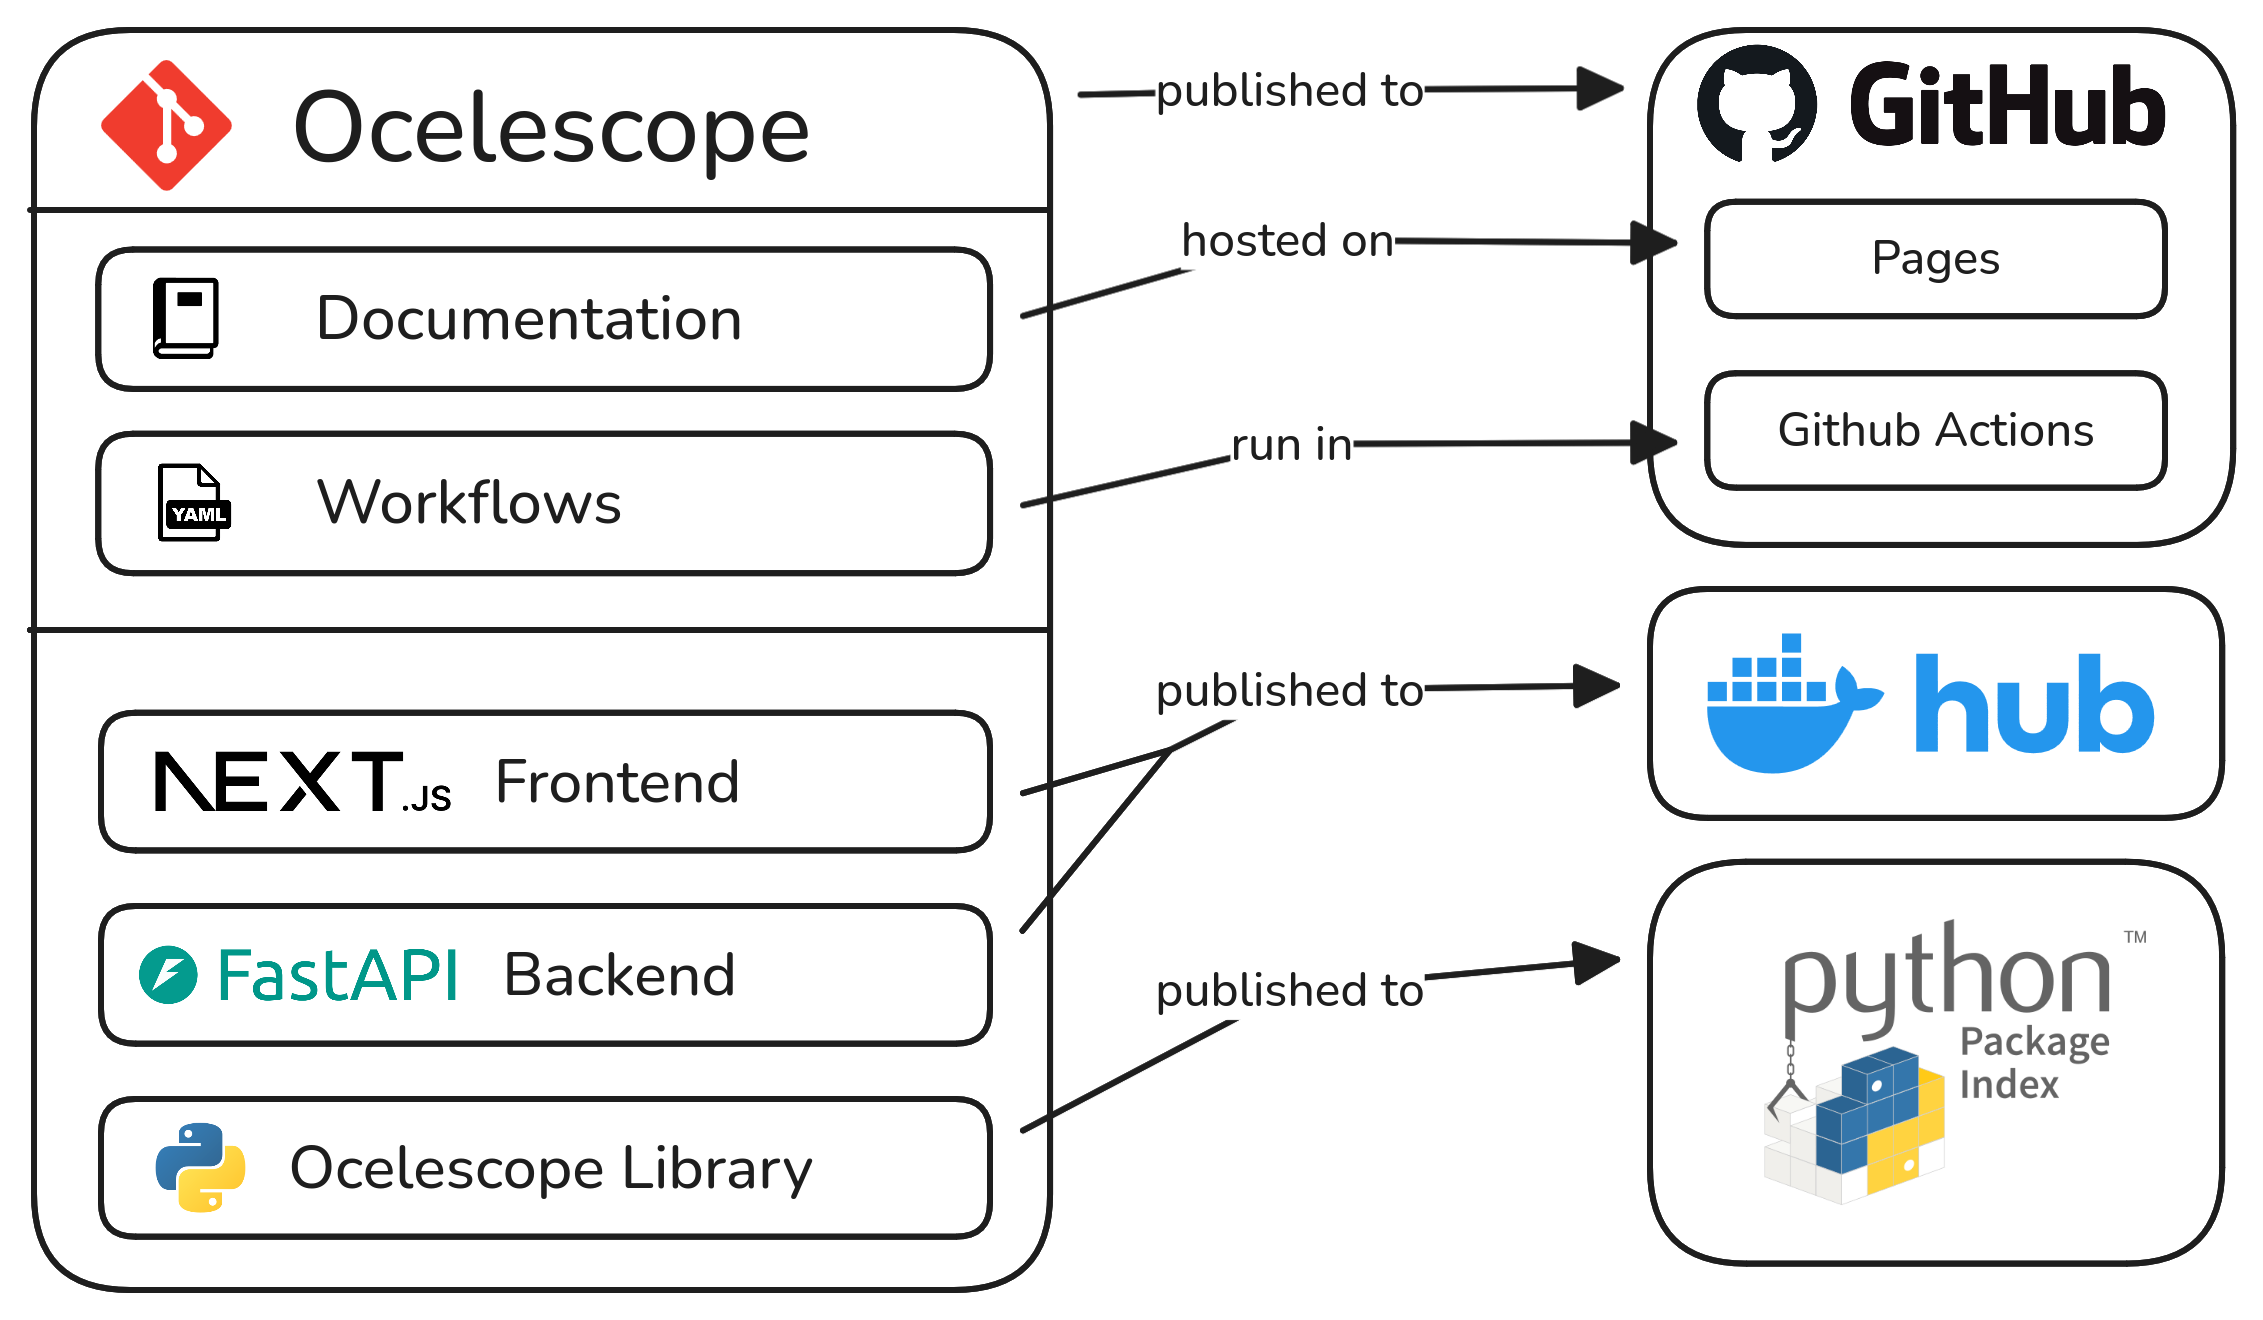
\includegraphics[width=0.6\linewidth]{./figures/implementation/RepoStructure.png}
	\caption{Overview of the \textit{Ocelescope} monorepo and its distribution targets.}
	\label{fig:repo_structure}
\end{figure}

\subsection{Backend}

The backend of \textit{Ocelescope} is implemented using FastAPI\footnote{\url{https://fastapi.tiangolo.com/}}, a popular framework for building REST APIs in Python.

As mentioned earlier, \textit{Ocelescope} works with user sessions to allow several users to work on the same instance.
A session stores all uploaded OCELs and all results produced by plugins.
OCELs are stored as wrapped \texttt{pm4py} OCEL objects, and resources are stored as JSON data.
Keeping all session data in memory makes interactions fast and keeps the infrastructure simple.

The backend provides a collection of base API endpoints that cover three main areas:

\begin{itemize}
	\item \textbf{Session Management:} Creating and managing sessions and handling the storage of OCELs and resources.
	\item \textbf{Basic OCPM Functions:} Providing simple functions that extract information from OCELs.
	\item \textbf{Plugin Management:} Listing available plugins and executing plugin functions.
\end{itemize}

OCPM often requires significant computation.
Importing or exporting large OCELs or running process discovery on large logs can take several minutes, as demonstrated in \cite{oclpm}.
To avoid blocking the user interface during such operations, \textit{Ocelescope} uses asynchronous tasks.
These tasks allow long-running operations to execute in the background while the frontend remains responsive.
Tasks are used, for example, when parsing uploaded OCELs and when executing plugins, which ensures that plugin execution does not block the application.
Many tools discussed in the previous chapter use the same default OCELs for evaluation.
For instance, \cite{textmining, silentobjects, occnet} all use the artificial event logs introduced in \cite{containerlogistics}.
For this reason, the backend includes several commonly used OCELs that can be loaded directly into a user session.
These logs are based on the examples published on the \textit{OCEL~2.0} standard website\footnote{\url{https://ocel-standard.org/event-logs/overview/}}.

\begin{figure}[ht]
	\centering
	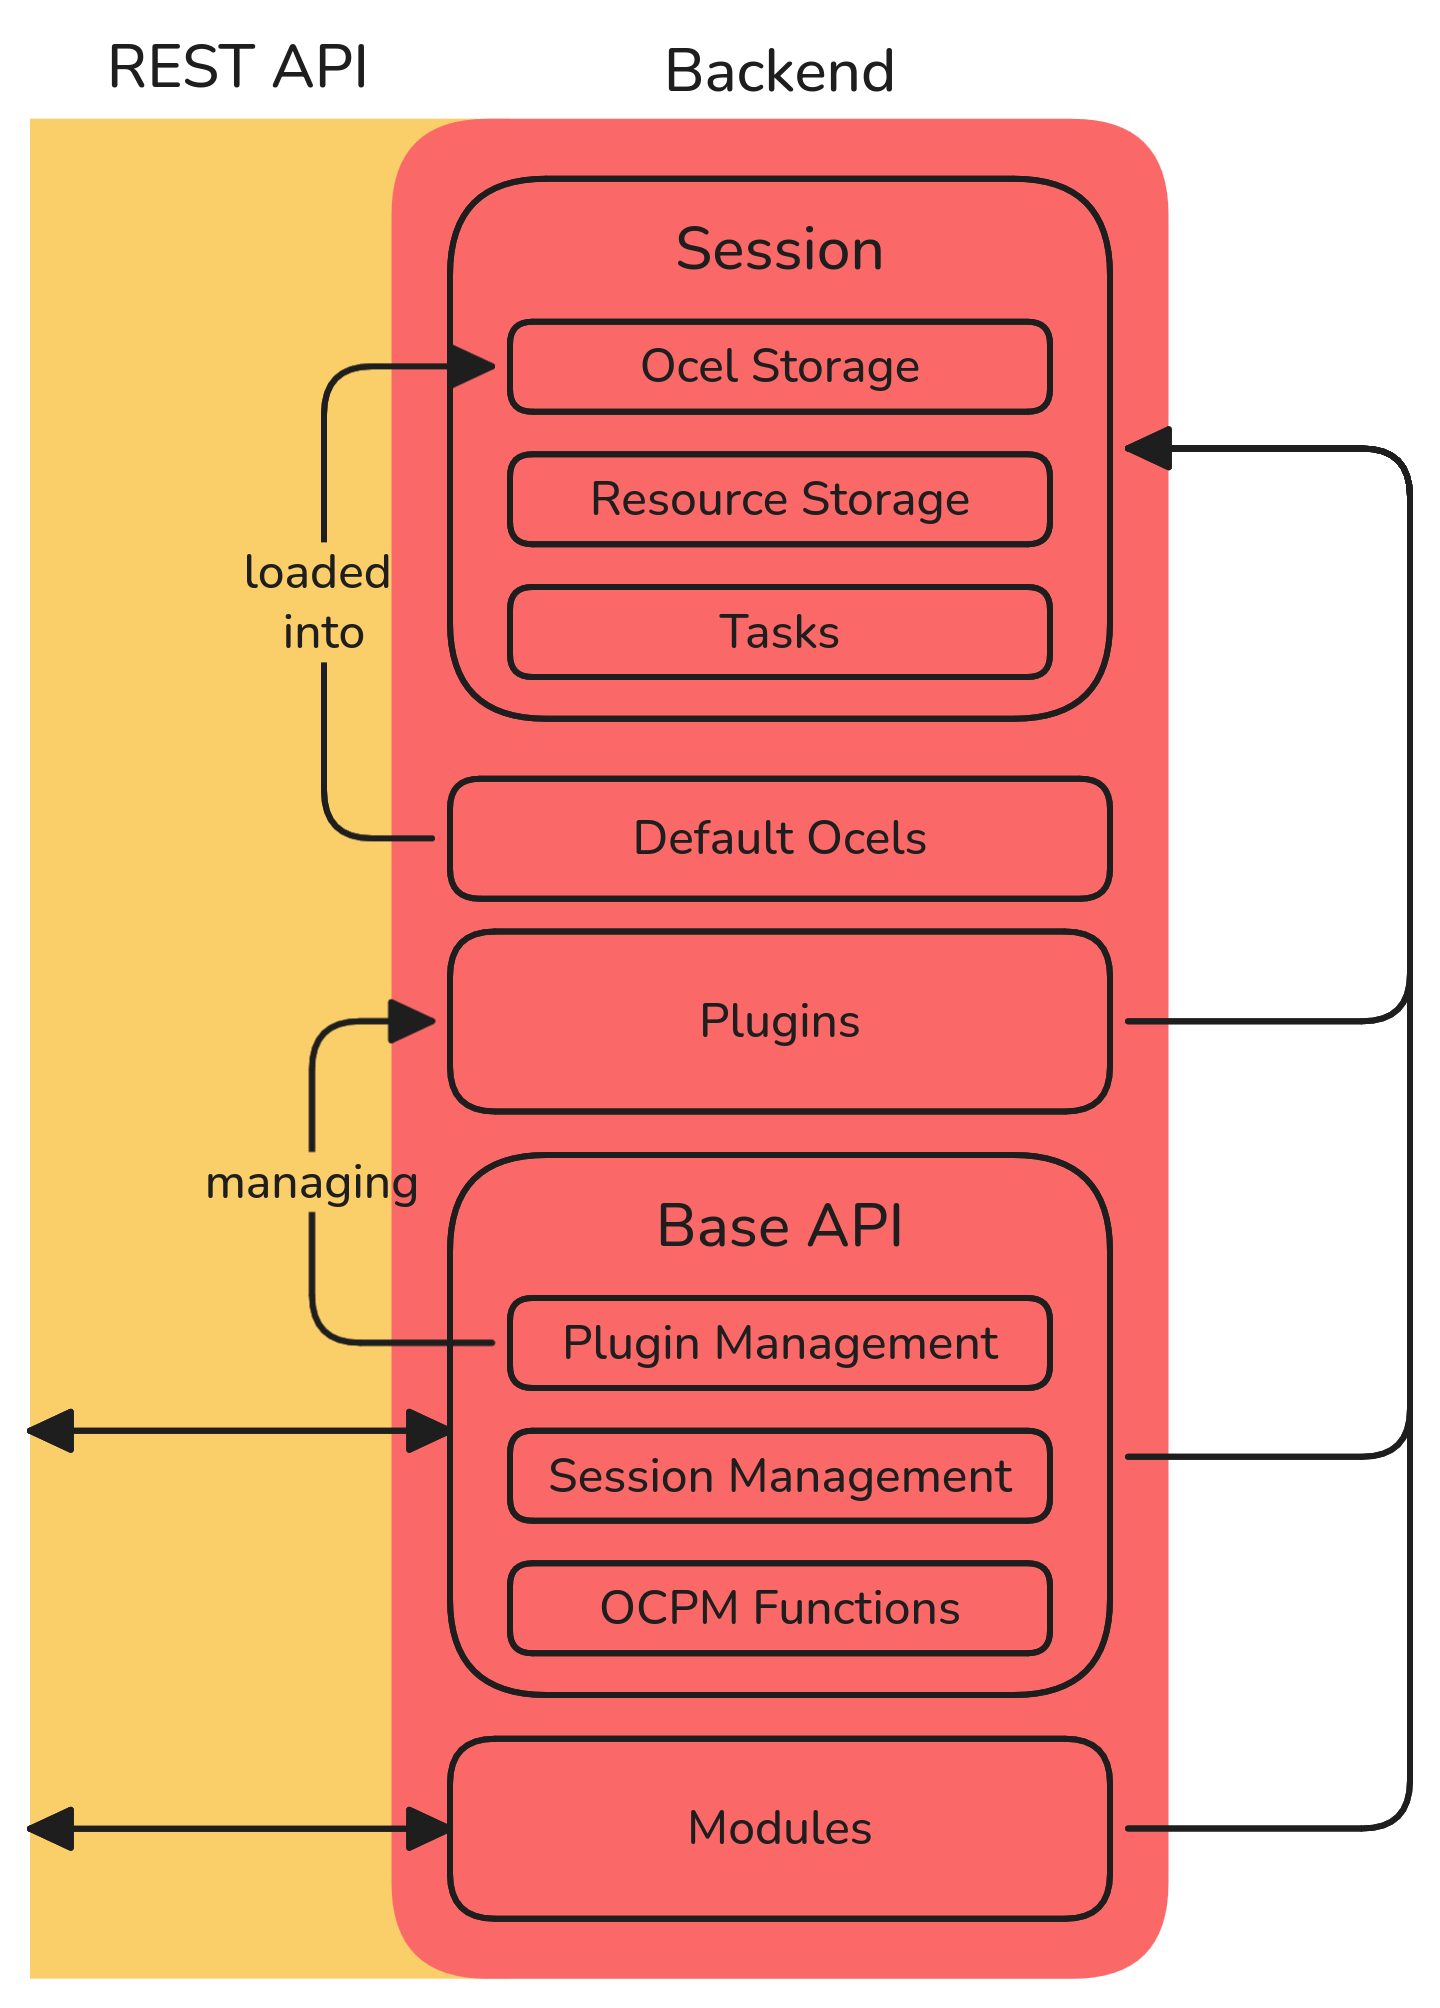
\includegraphics[width=0.4\textwidth]{./figures/implementation/Backend.png}
	\caption{Overview of the backend structure in \textit{Ocelescope}.}
	\label{fig:backend-overview}
\end{figure}

\subsection{Frontend}

The frontend of \textit{Ocelescope} is implemented using the commonly used React framework Next.js\footnote{\url{https://nextjs.org/}}.
To keep the interface coherent and to support less experienced developers, the Mantine\footnote{\url{https://mantine.dev/}} component library is used. Mantine provides many ready-to-use components and supports consistent styling and theming.
The user interface is embedded in an app shell. Navigation is handled through a sidebar, which links to the session management interface, the plugin interface, and all views provided by frontend modules. The session management interface serves as the default home view. Users can upload OCELs and resources, inspect them, rename them, and delete them. The interface also shows an overview of all uploaded plugins.

\begin{figure}[ht]
	\centering
	\begin{subfigure}[t]{0.48\textwidth}
		\centering
		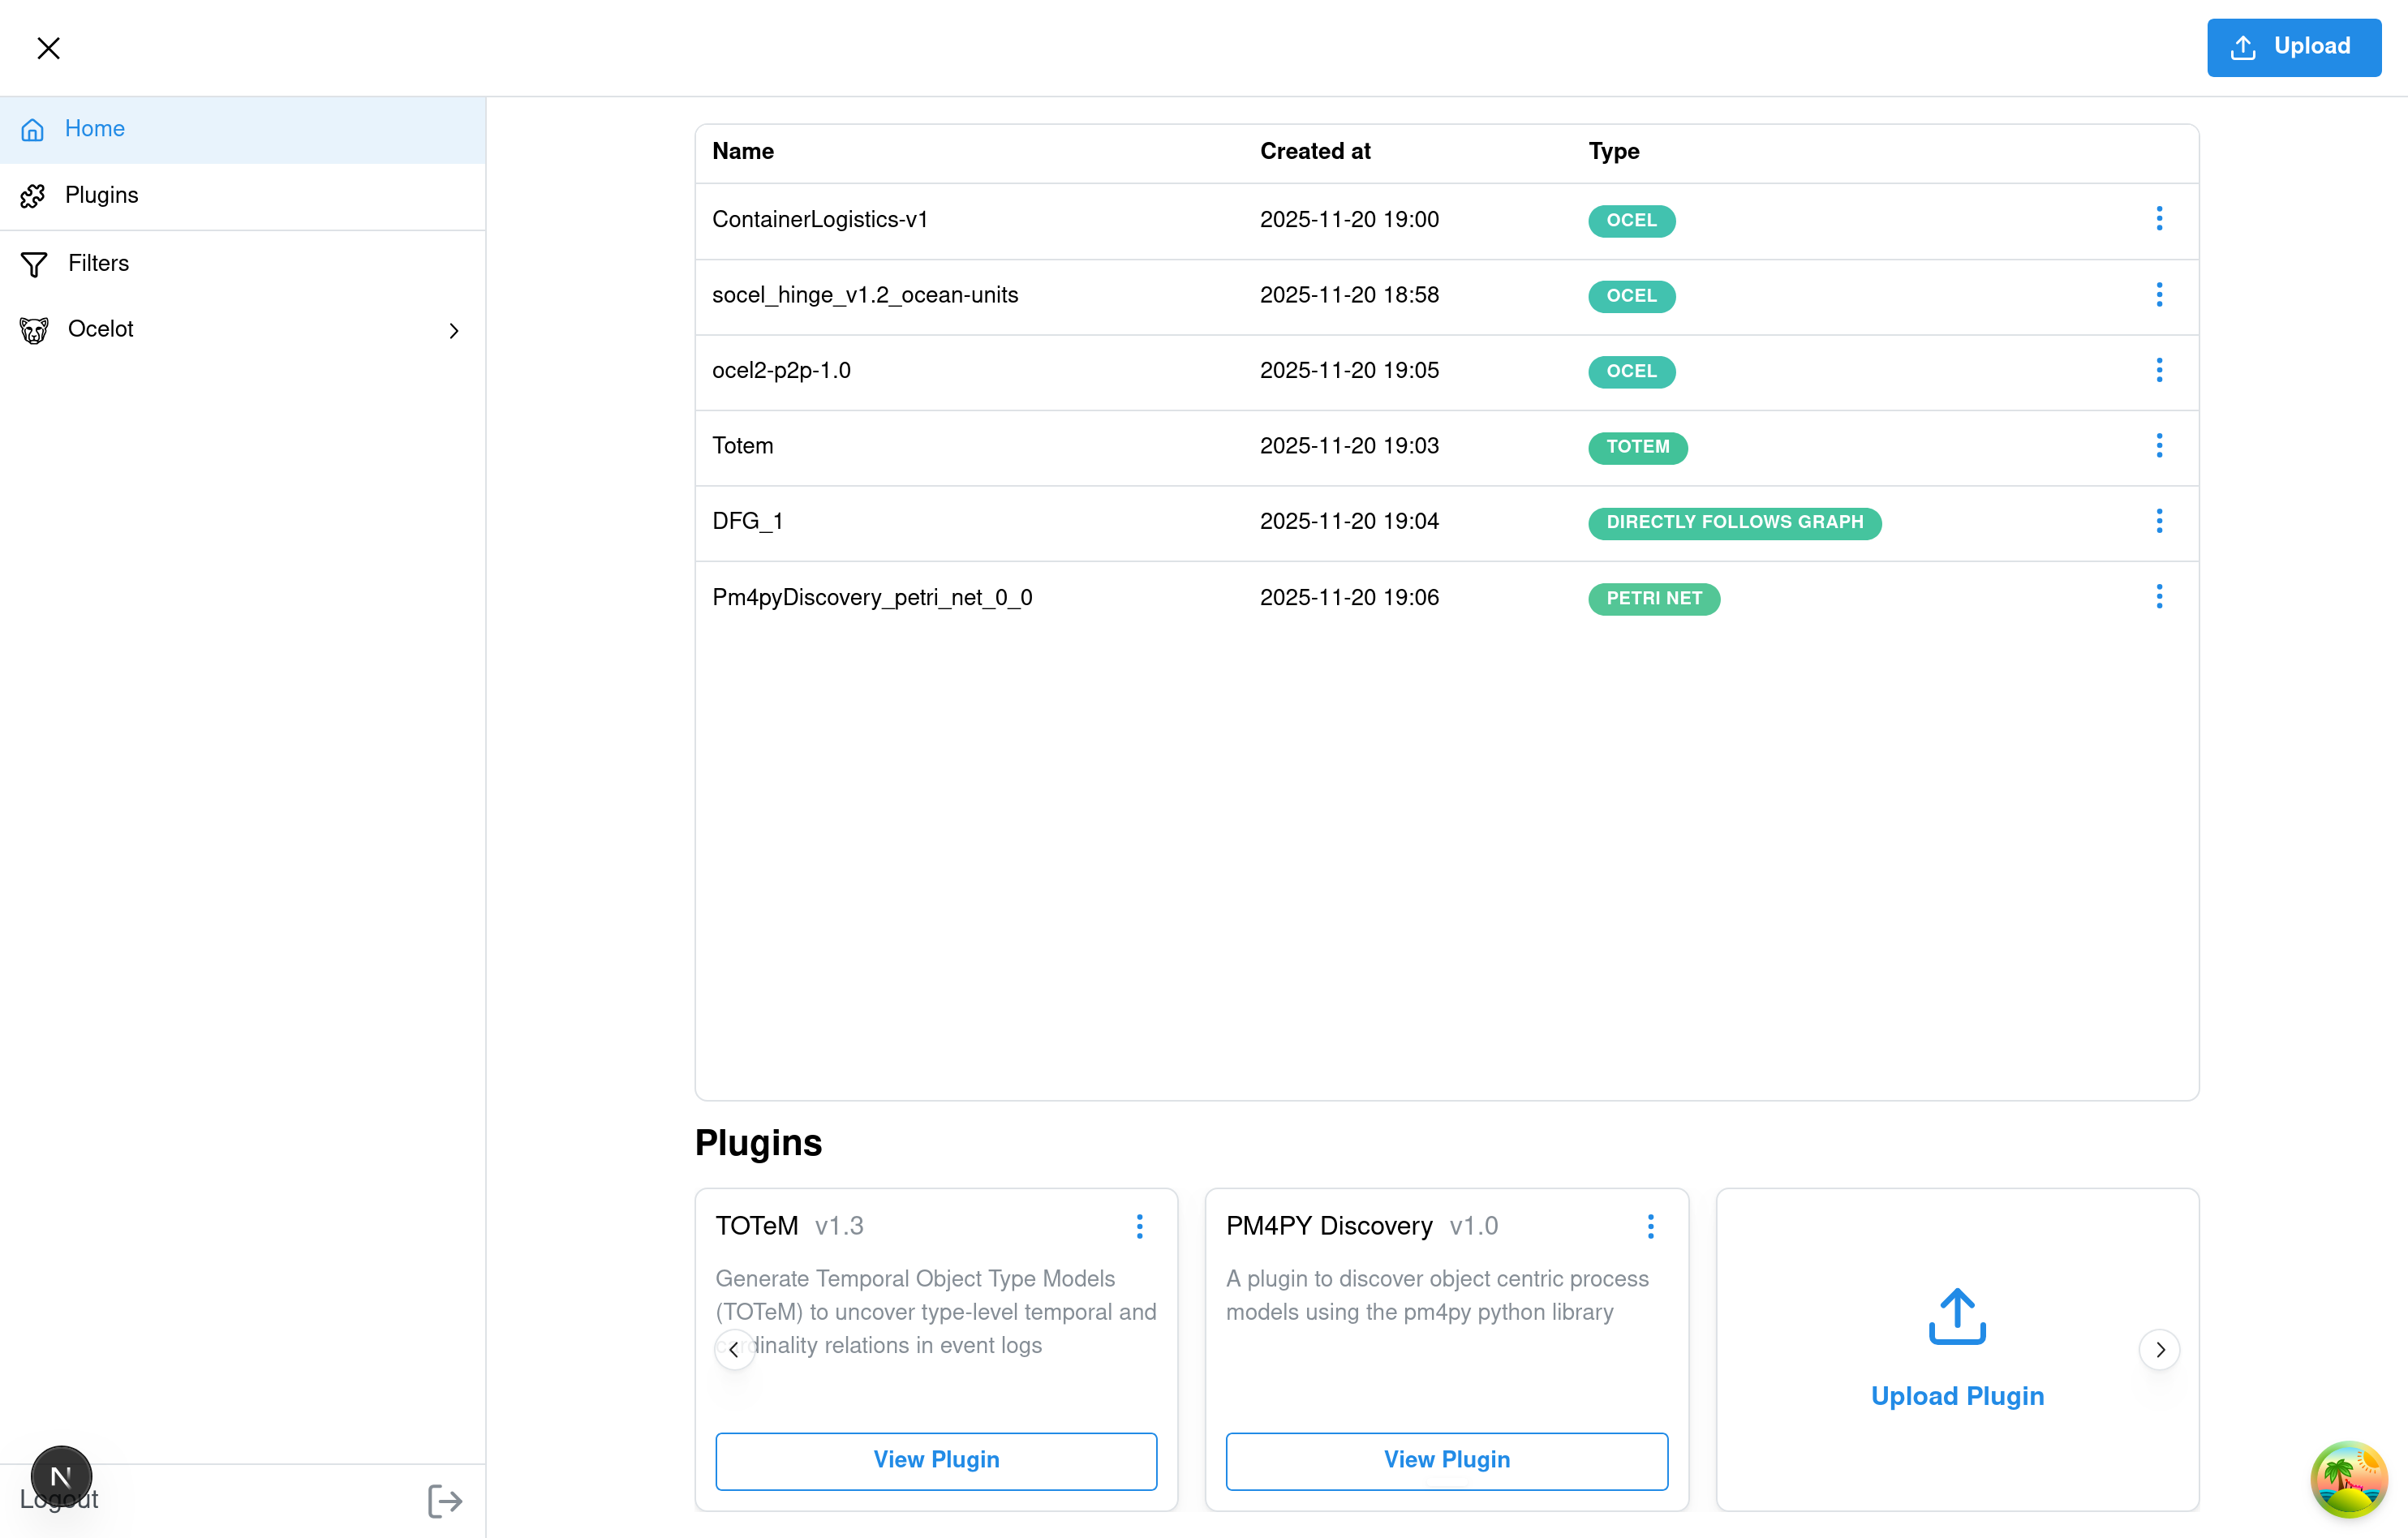
\includegraphics[width=\textwidth]{./figures/implementation/SessionManager.png}
		\caption{Session management interface.}
		\label{fig:frontend-session}
	\end{subfigure}
	\hfill
	\begin{subfigure}[t]{0.48\textwidth}
		\centering
		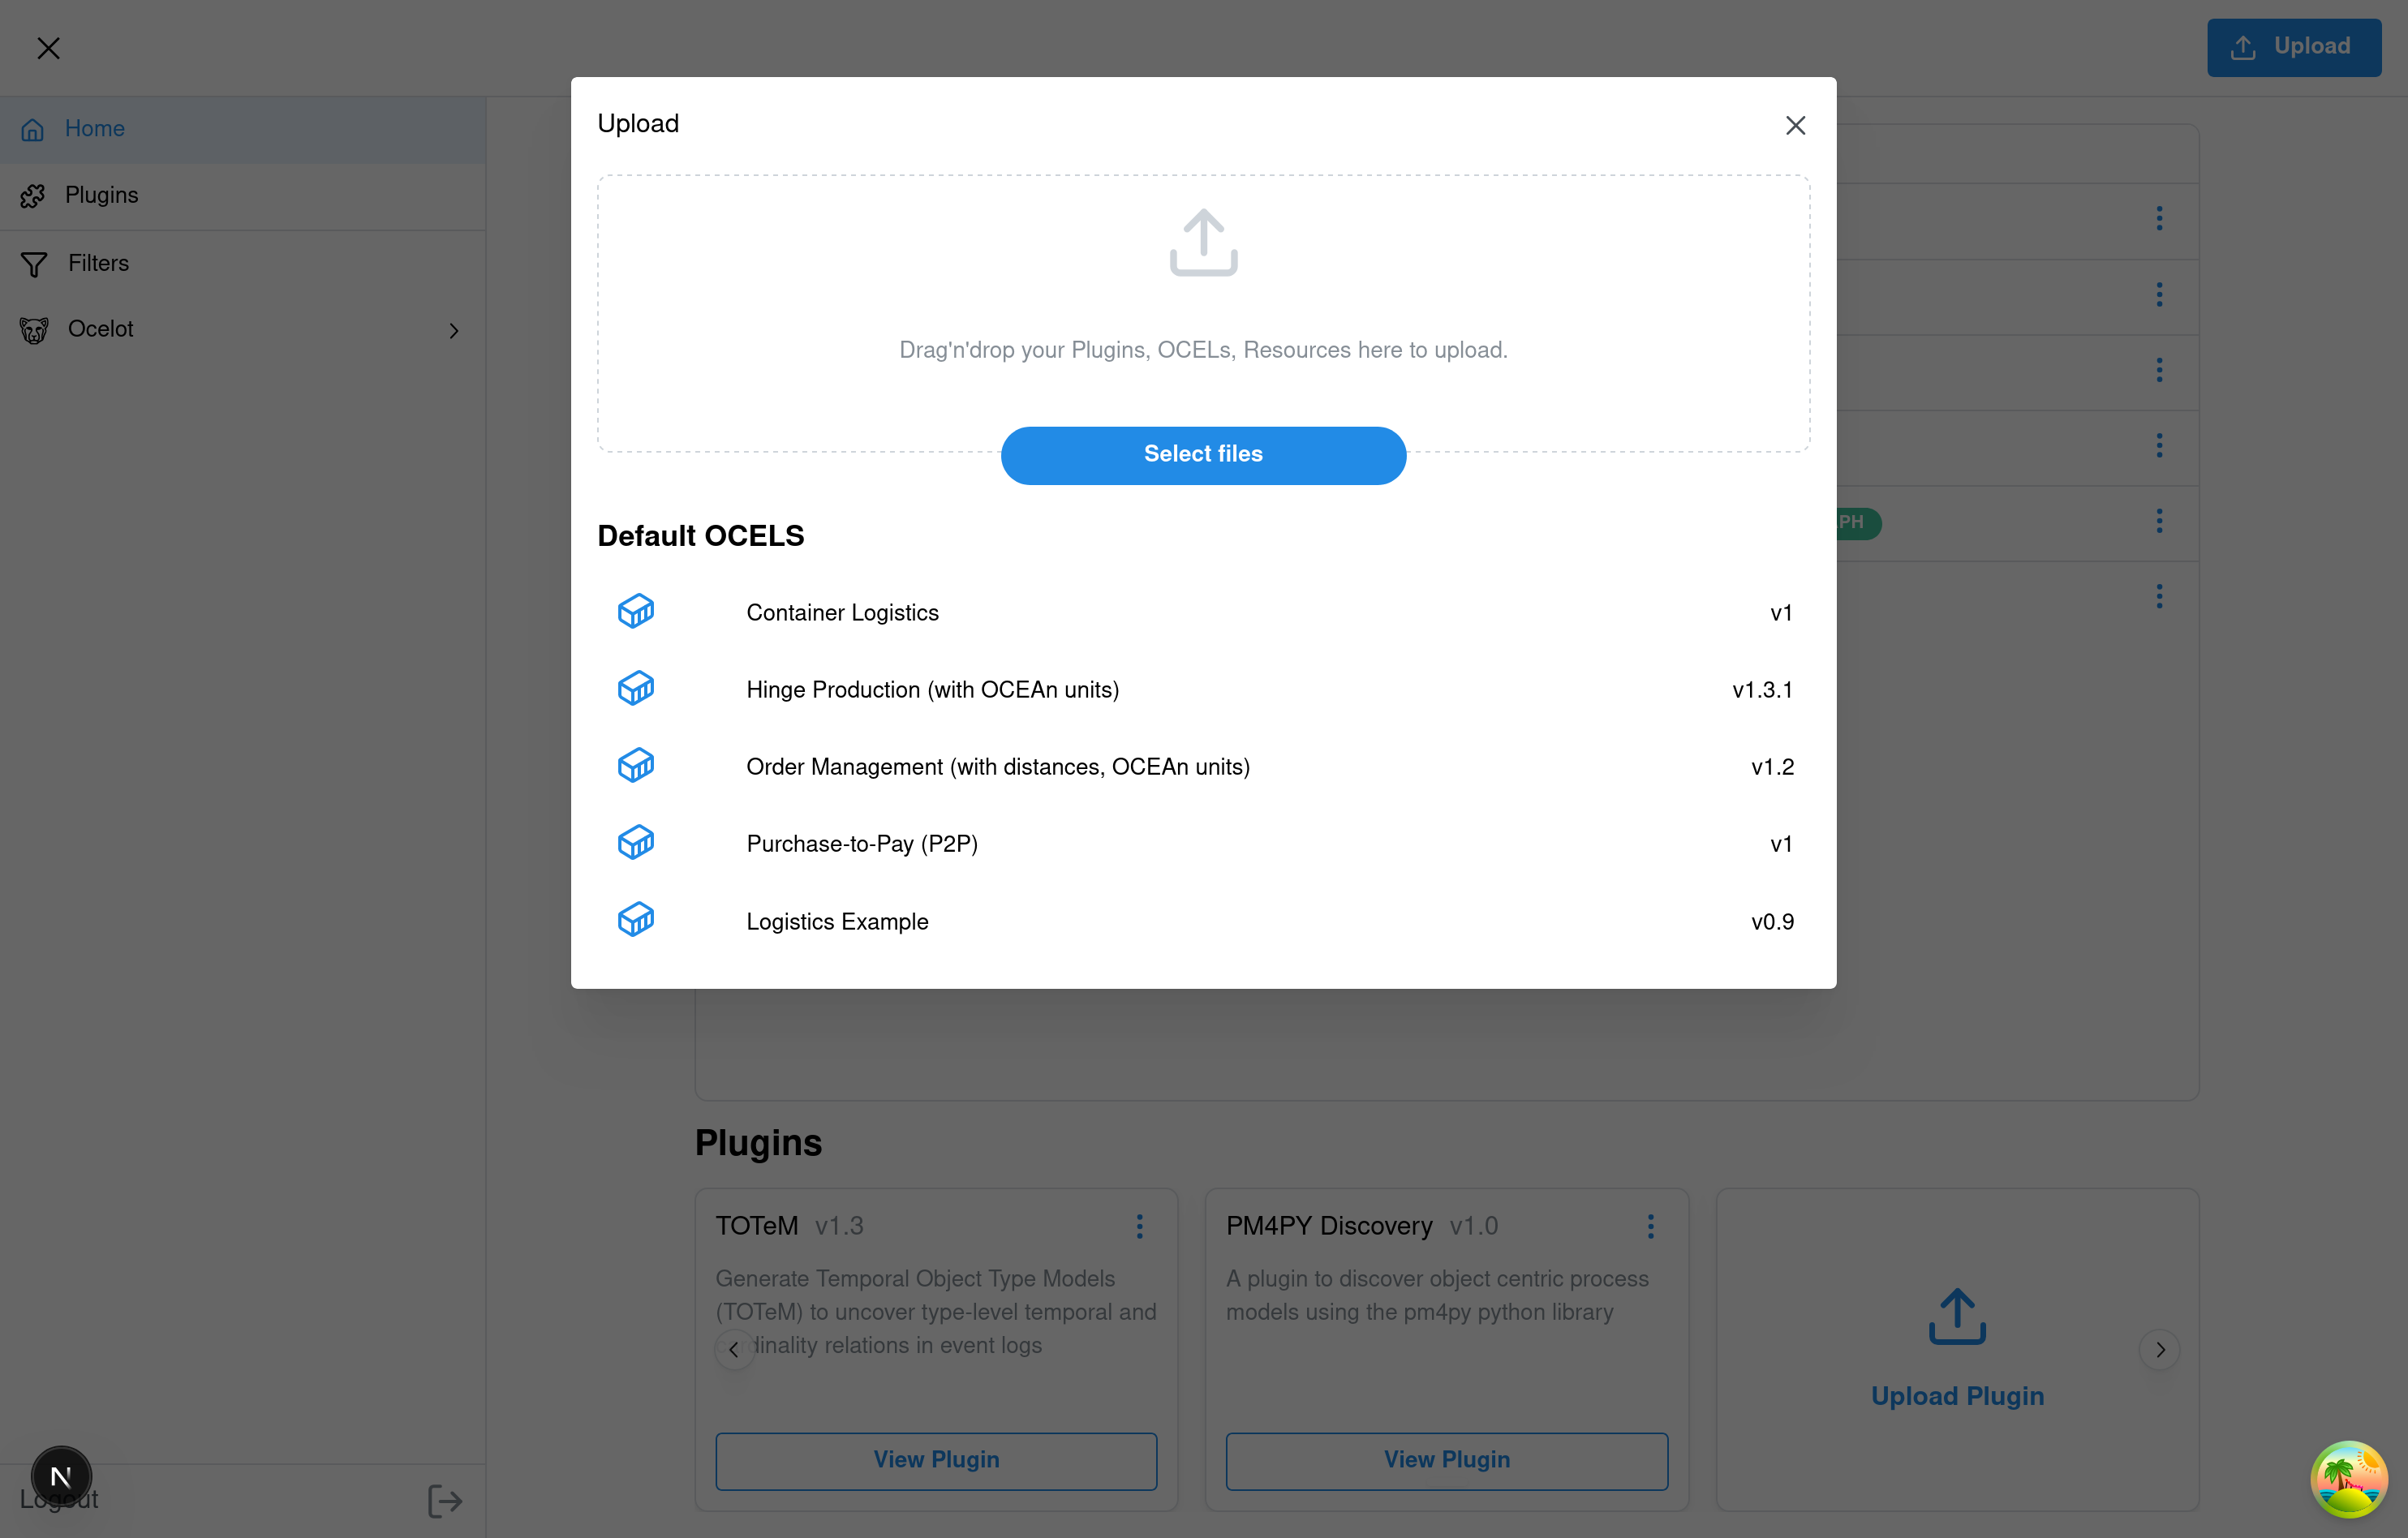
\includegraphics[width=\textwidth]{./figures/implementation/Upload.png}
		\caption{Upload dialog with default OCELs.}
		\label{fig:frontend-upload}
	\end{subfigure}
	\caption{Frontend views in Ocelescope.}
	\label{fig:frontend-overview}
\end{figure}

\subsection{Communication Between Frontend and Backend}

As described in \cref{chap:design}, the frontend and backend communicate through REST APIs.
To simplify this communication, the frontend uses a client generator based on the OpenAPI schema of the backend.
This allows both framework developers and module developers to call backend functions in an ergonomic and type-safe way.
The generated clients also support caching, which prevents identical process mining tasks from being executed multiple times.

\begin{figure}[ht]
	\centering
	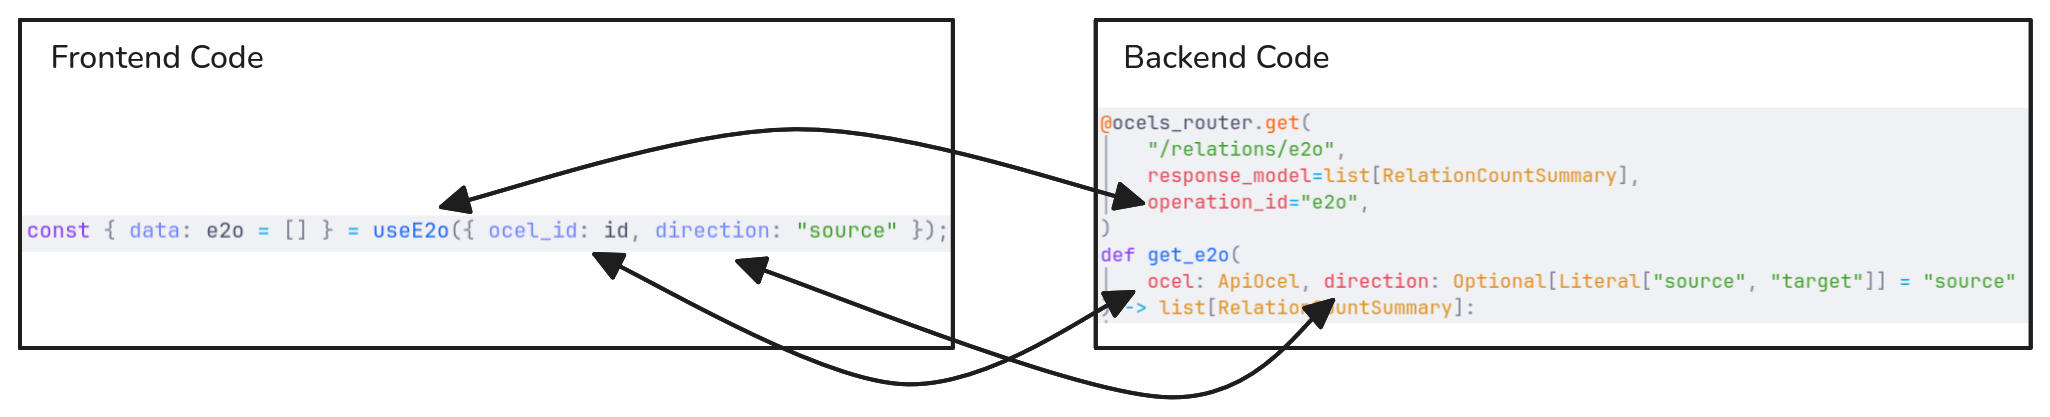
\includegraphics[width=\textwidth]{./figures/implementation/APIClientGenerator.png}
	\caption{Generated React Query hooks in the frontend and the corresponding backend endpoint.}
	\label{fig:api-generation}
\end{figure}

Each user session also opens a server-sent event connection to the backend.
This connection is used to send notifications and to invalidate cached data when results change.

\section{Ocelescope Python Library}

To develop plugins, developers must implement the plugin interfaces provided by \textit{Ocelescope}.
These interfaces are defined in a Python library that is distributed as a package on PyPI, allowing it to be easily installed and used.

Since neither \textit{OCPA}~\cite{ocpa} nor \textit{pm4py}~\cite{pm4py} provides comprehensive support for OCPM in Python, the \textit{Ocelescope} library additionally offers general OCPM functionality to address this gap.

\begin{figure}[ht]
	\centering
	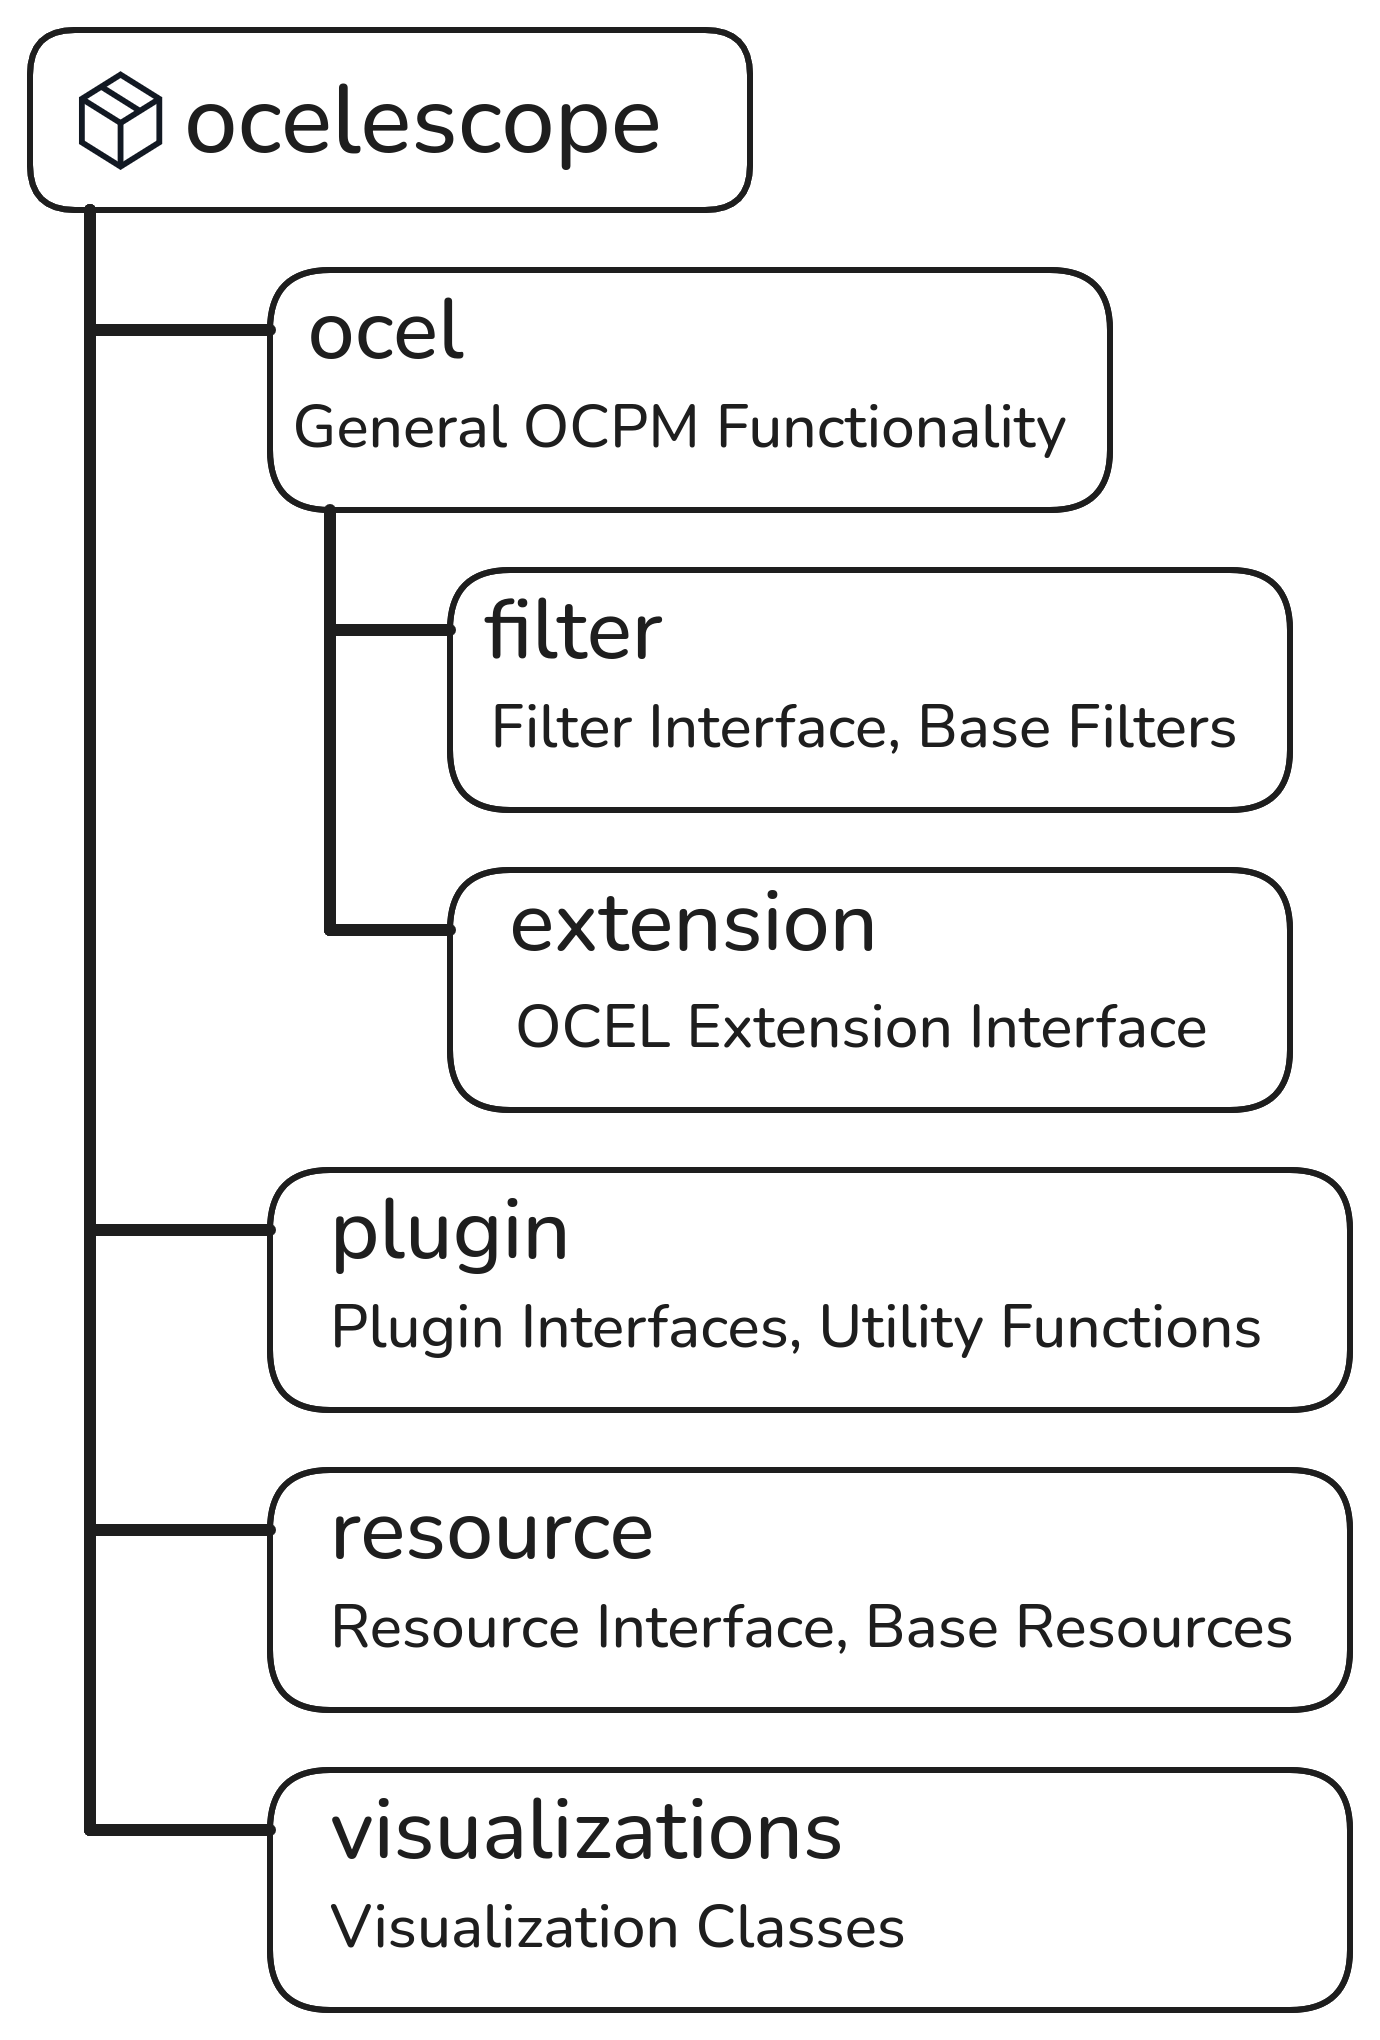
\includegraphics[width=0.3\textwidth]{figures/implementation/PackageStructure.png}
	\caption{Structure of the \textit{Ocelescope} Python package.
		Each submodule provides a dedicated part of the plugin API and supports both plugin development and standalone OCEL processing.}
	\label{fig:ocelescope-package-structure}
\end{figure}

\subsection{OCEL Class}

The main entry point for OCPM functionality is the \texttt{OCEL} class, which represents an instantiated OCEL. This class wraps the OCEL implementation provided by \textit{pm4py} and extends it with additional utility functions and cached properties.

Placing these utility functions directly in the \texttt{OCEL} class would result in a large and overly complex structure that combines too many responsibilities, commonly referred to as a god class~\cite{god-class}. To avoid this, the implementation is structured into dedicated subclasses that handle events, objects, event-to-object (E2O) relations, and object-to-object (O2O) relations. Each of these subclasses encapsulates functionality related to its respective part of the OCEL metamodel.

This design provides two main advantages. First, it improves maintainability by introducing a clear internal structure, which makes it possible to extend the implementation without introducing breaking changes. Second, it enables more intuitive access to OCEL properties by grouping related functionality in a consistent way.

Although the \textit{Ocelescope} package includes documentation, the core functionality is implemented to be discoverable without consulting it. This distinguishes the library from other Python-based OCPM tools, where basic tasks typically require consulting documentation.

\paragraph{Filters.}
The Python package also provides functionality for filtering OCELs. Filters are not defined as standalone functions. Instead, they are implemented as classes that follow a shared filtering interface. Each filter class defines its parameters and implements a filtering function that takes an OCEL as input.

The filtering function does not create a new OCEL directly. Instead, it produces boolean masks for events, objects, and relations. Each mask assigns a boolean value to an entity and indicates whether the entity should be retained in the filtered log.

Multiple filter instances can be combined into a filter pipeline. Each filter contributes its own masks, and these masks are combined using a logical $\land$ operation. An entity is retained only if all masks evaluate to true. After applying the combined masks, the resulting OCEL is validated and cleaned to remove invalid structures.

\begin{figure}[ht]
	\centering
	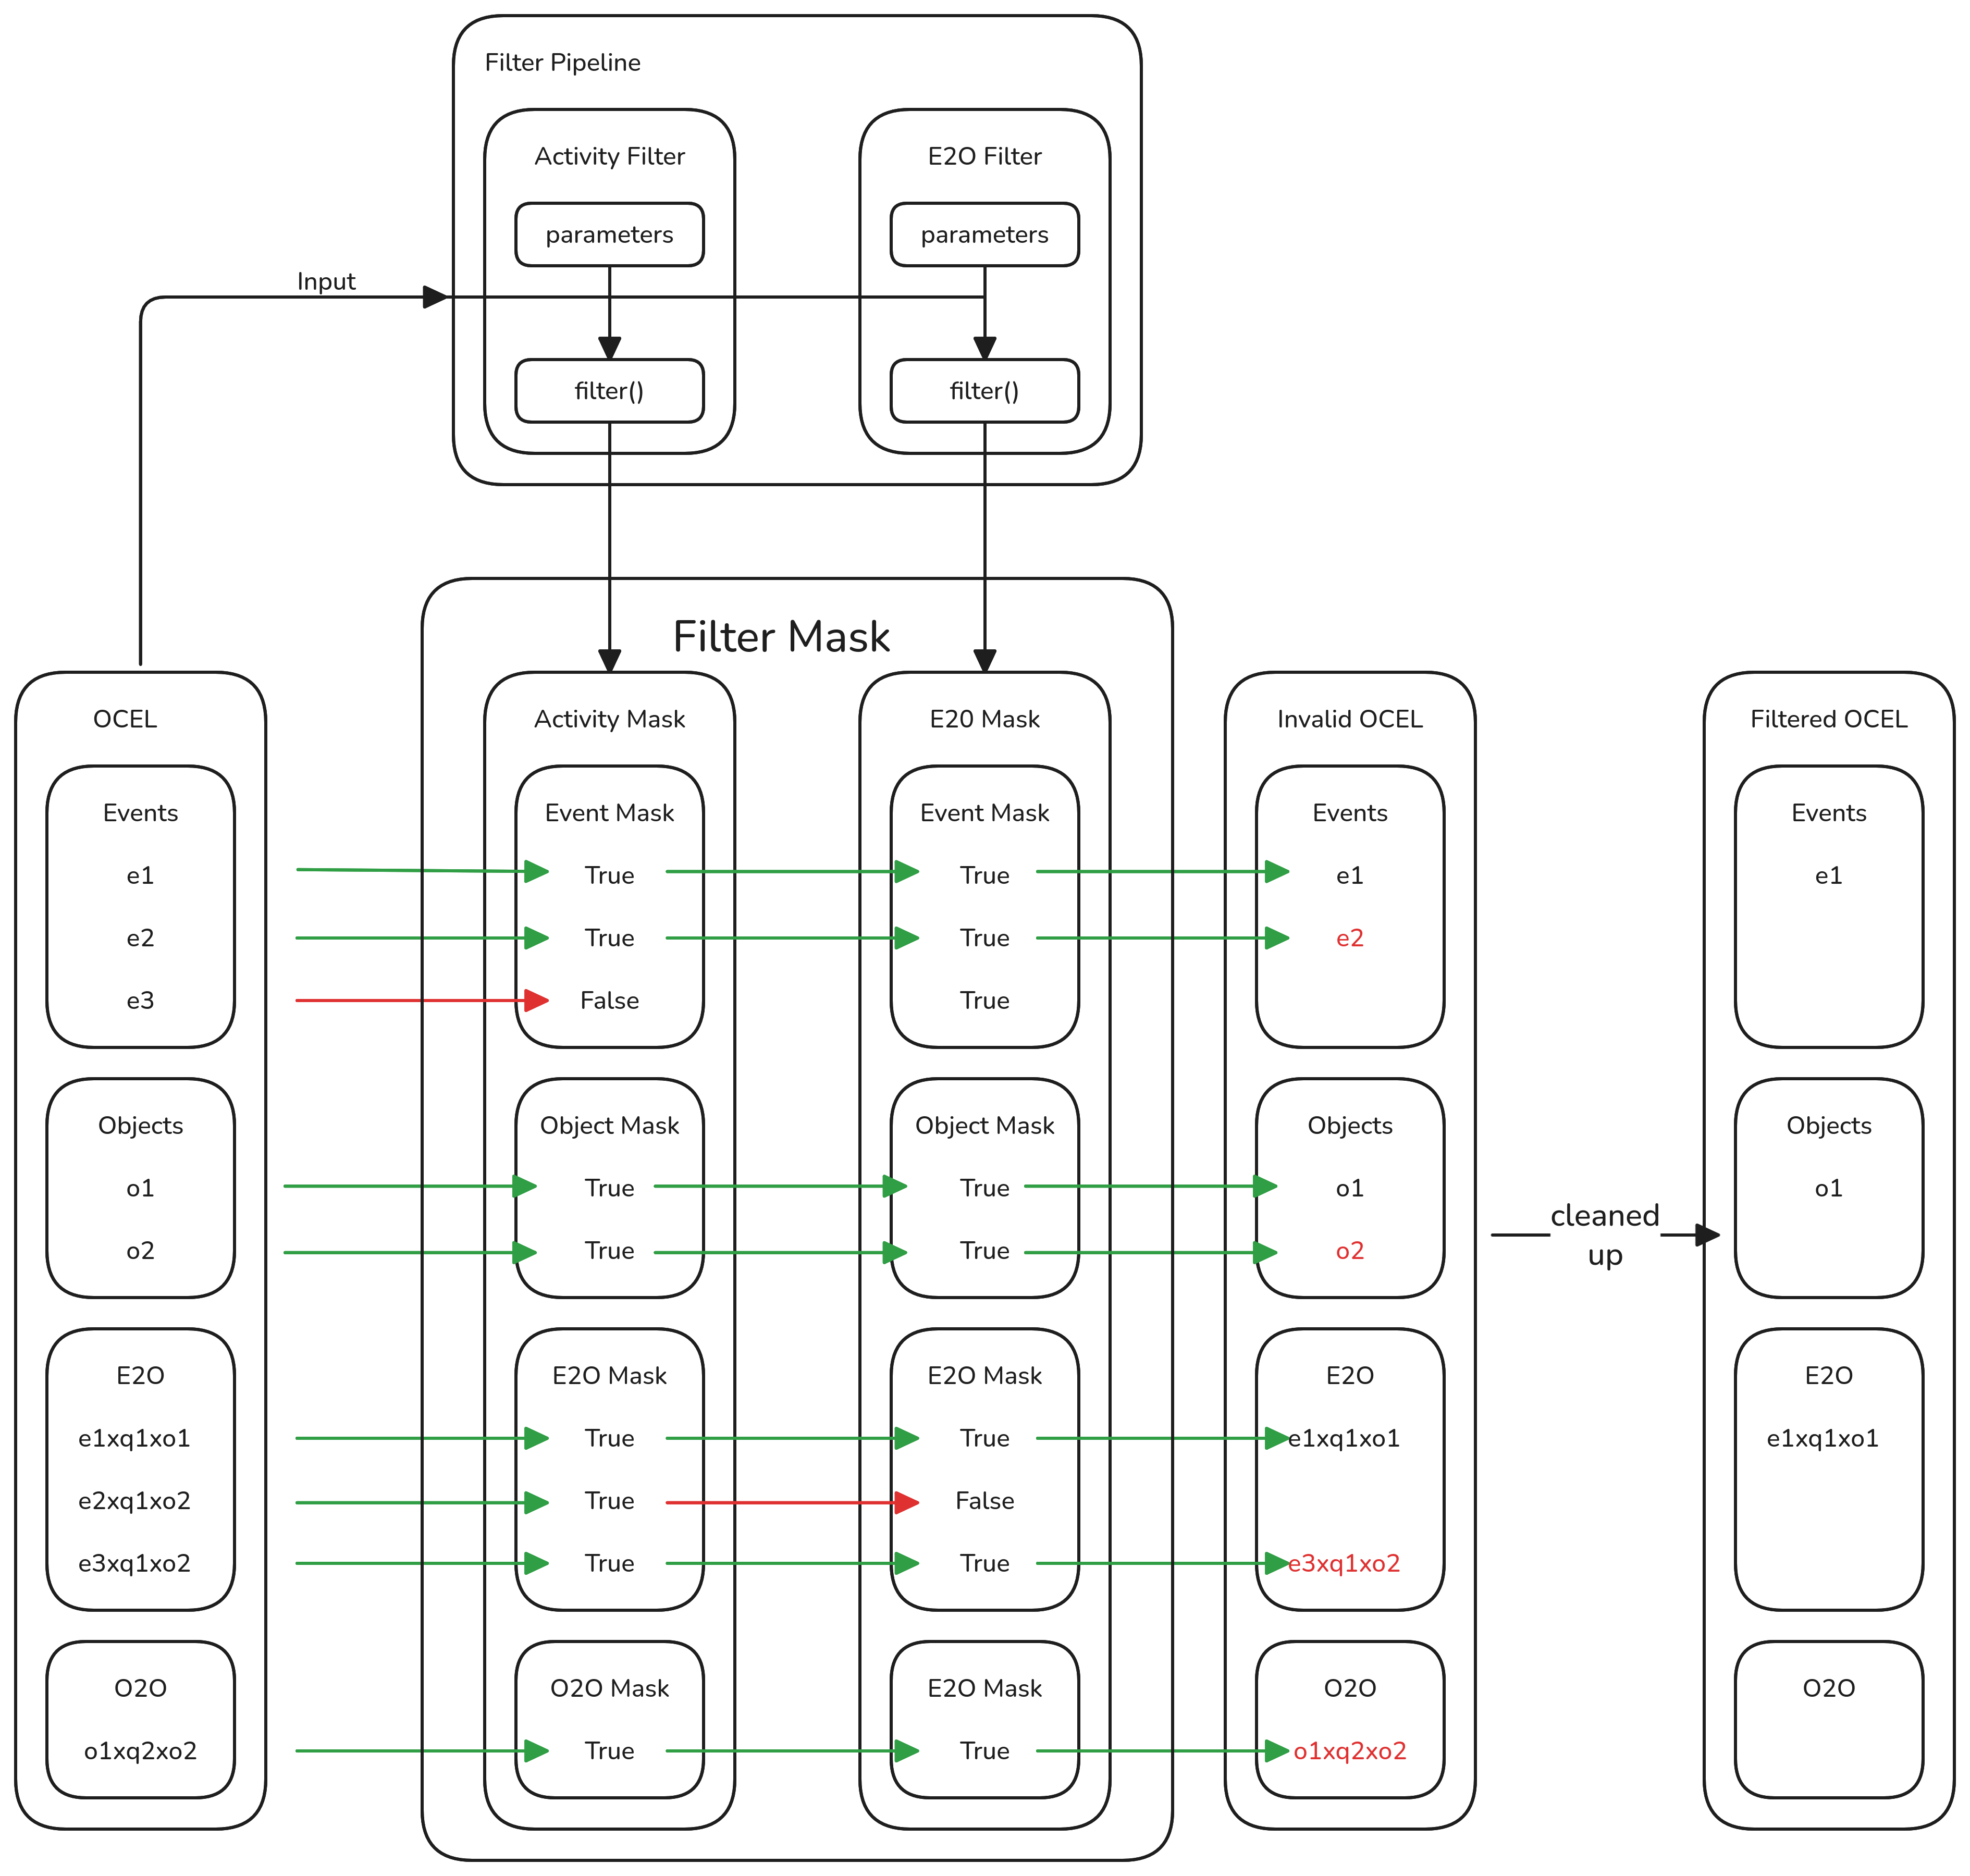
\includegraphics[width=0.55\textwidth]{figures/design/Filter Pipeline V1.png}
	\caption{Filtering process in \textit{Ocelescope}.
		Each filter produces boolean masks for events, objects, and relations.
		Masks from several filters are combined in a pipeline, and invalid elements are removed during cleanup.}
	\label{fig:filter-pipeline}
\end{figure}
During this cleanup step, the following elements are removed:

\begin{itemize}
	\item events that are not related to at least one object,
	\item objects that are not related to an event or another object,
	\item relations whose referenced entities do not exist in the filtered log.
\end{itemize}

This design makes filters composable and easy to extend.
Developers can implement custom filters that work together with the existing ones and can contribute them to the main package if the functionality is generally useful.

The \textit{Ocelescope} package provides classes for all filters defined in Section~\ref{sec:filtering}.

\section{Plugins Implementation}
\label{sec:plugins-imp}

Plugins in \textit{Ocelescope} are implemented as Python modules and are distributed as ZIP archives.
They are created using base classes provided by the \textit{Ocelescope} package.
The plugin mechanism is kept simple so that prototypes created during experimentation can be turned into plugins with little effort and with as little required knowledge as possible.

The goal of the design is to keep plugin development familiar to researchers.
Plugins should be easy to add after the main experimentation phase and should not require learning many new concepts.

\subsection{Automatic Schema Generation with Pydantic}

Both resources and plugin inputs require the definition of JSON Schema.
While JSON data is simple in structure, JSON Schema is more complex to write and understand. It is not intuitive to write and requires familiarity with its structure and constraints.
Since plugin and module development should require as little additional knowledge as possible, \textit{Ocelescope} uses Python classes to define these structures instead of writing JSON Schema manually.

This is achieved using the Pydantic\footnote{\url{https://docs.pydantic.dev/}} library.
Pydantic is widely used in web frameworks for data validation.
It provides a base model that allows inheriting classes to generate JSON Schema automatically.
Developers therefore define plugin inputs, resources, and other structured data using familiar Python type annotations, while Pydantic generates the corresponding JSON Schema in the background.

\begin{figure}[h]
	\centering
	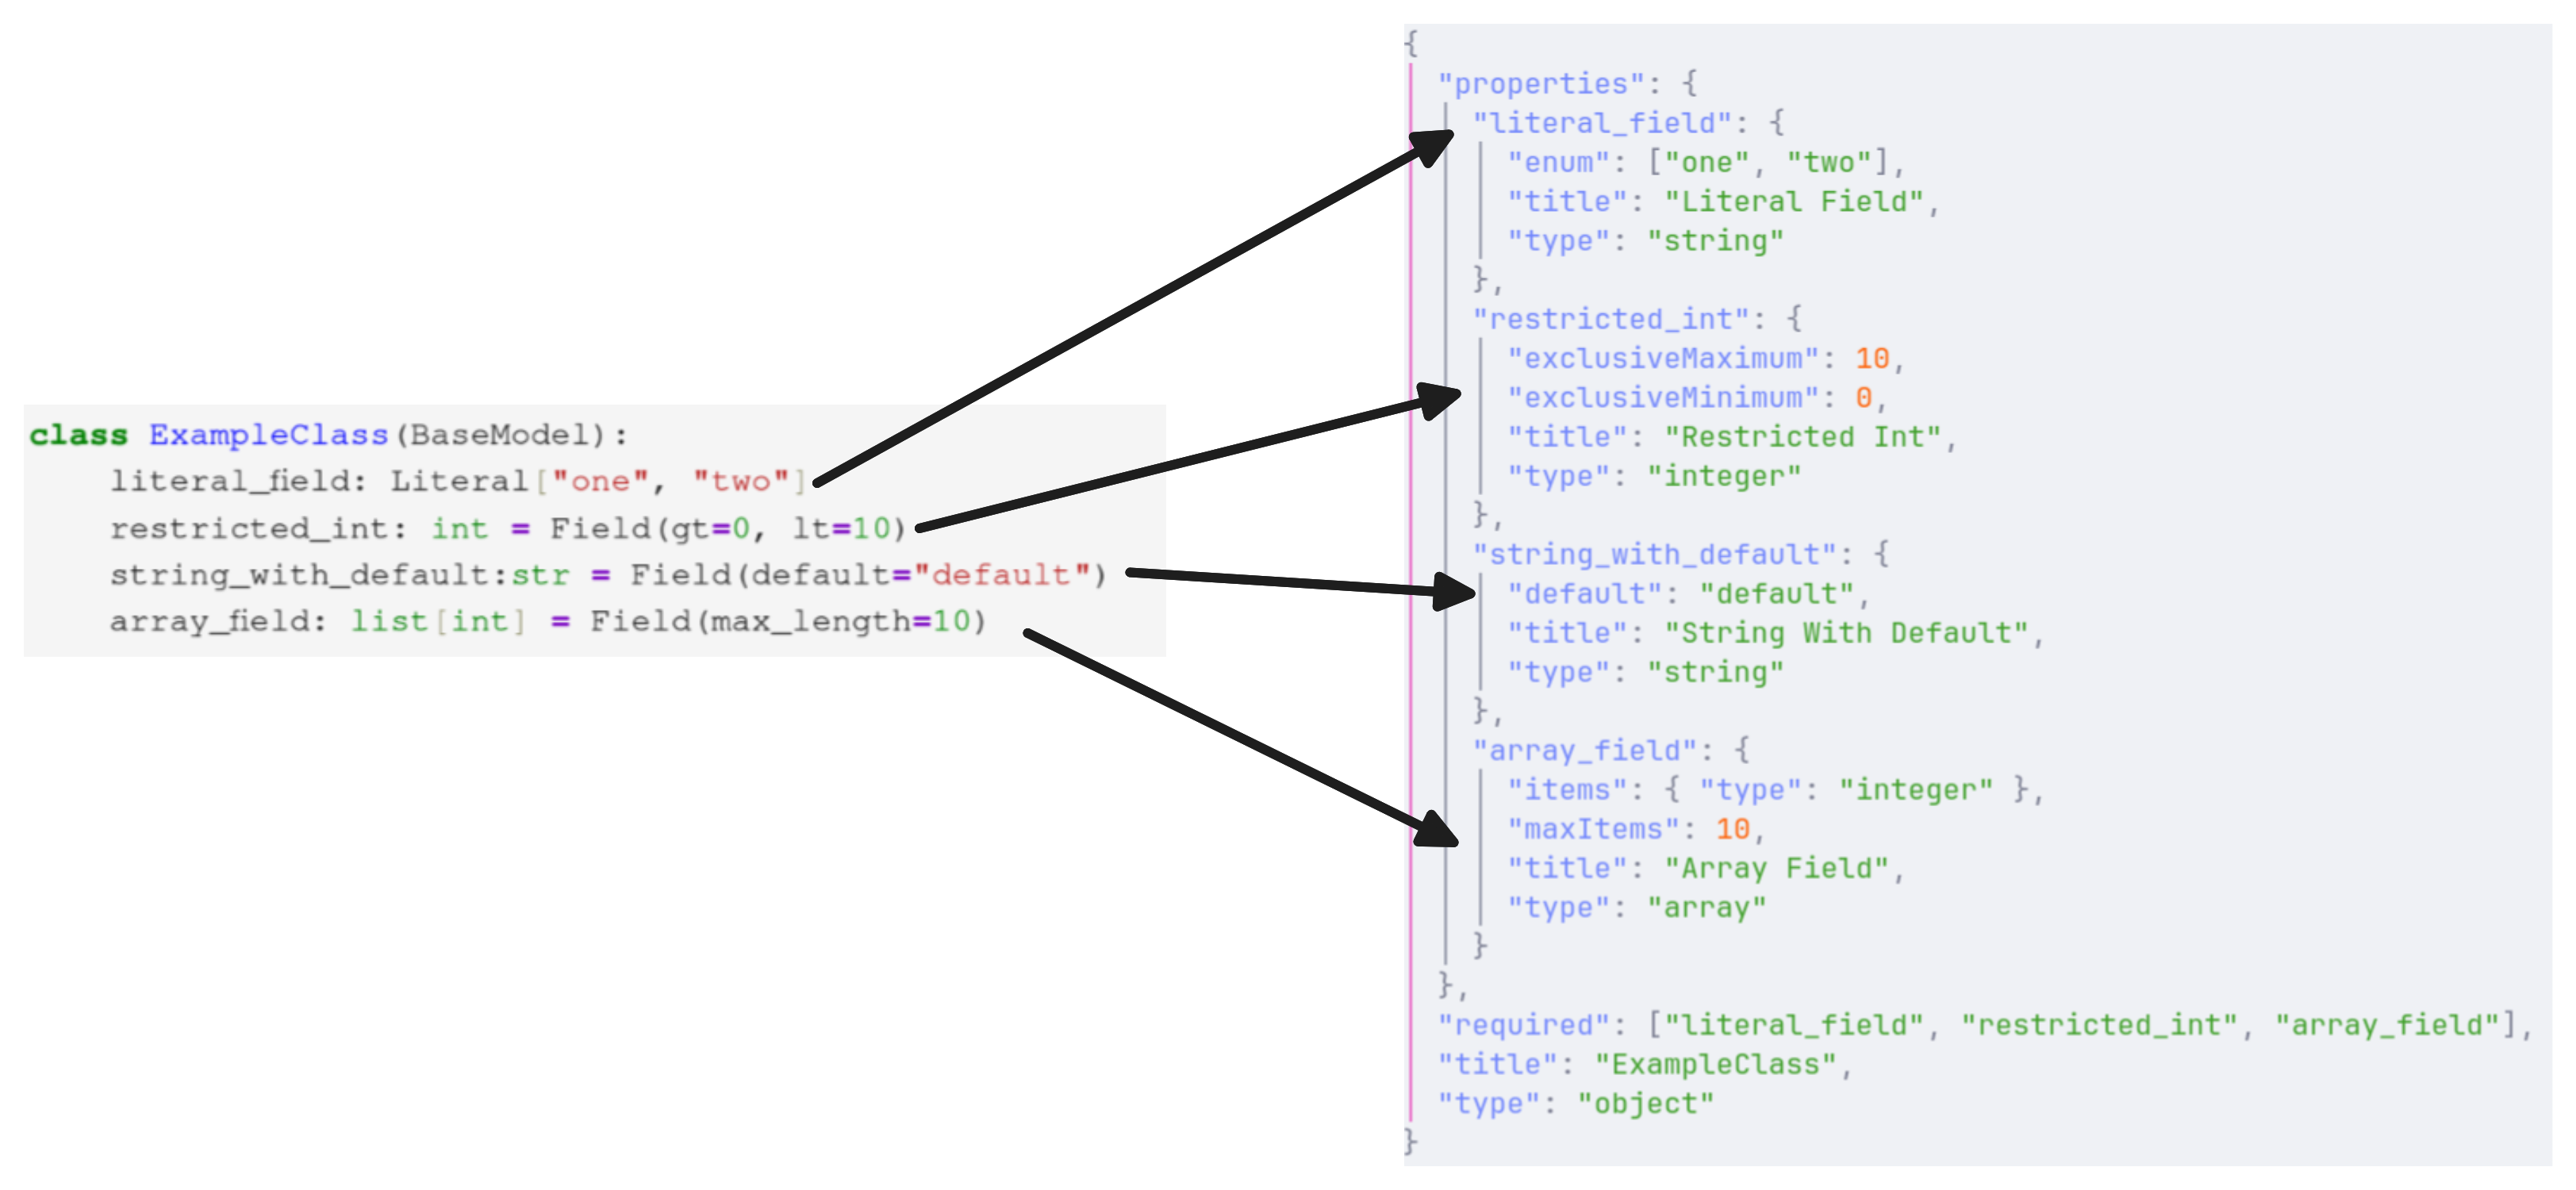
\includegraphics[width=0.8\textwidth]{figures/implementation/pydanticusecase.png}
	\caption{A Pydantic class and the JSON Schema automatically generated from it.
		Pydantic converts Python type annotations into complete and valid JSON Schema definitions.}
	\label{fig:pydantic-schema}
\end{figure}

Pydantic also provides helper functions for defining constraints on fields.
Examples include restricting integers to specific ranges or limiting the size of arrays.
Although this approach introduces a few additional concepts, the library provides a reasonable compromise compared to defining JSON Schema from scratch.

\subsection{Resources}

Resources implement the \texttt{Resource} base class provided by the \textit{Ocelescope} package.
They define their metadata through class variables and specify their fields as class properties.
A resource may also implement a \texttt{visualize} function that maps its instances to visualization classes from the visualization module (see \cref{tab:ocelescope-visualization-types}).
Each type has a dedicated viewer in the frontend.

\begin{table}[ht]
	\centering
	\caption{Visualization types supported by the visualization module.}
	\label{tab:ocelescope-visualization-types}
	\begin{tabular}{p{0.17\textwidth} p{0.78\textwidth}}
		\hline
		\textbf{Type} & \textbf{Description}                                                                                          \\
		\hline
		Table         & A table rendered from a list of Python dictionaries.                                                          \\
		SVG           & A vector graphic rendered from an SVG string.                                                                 \\
		Plotly        & An interactive chart created using the charting library \textit{Plotly}.                                      \\
		DOT           & A graph rendered with \textit{Graphviz} from the DOT language.                                                \\
		Graph         & An interactive graph rendered from custom \texttt{Graph} classes provided by the \textit{Ocelescope} package. \\
		\hline
	\end{tabular}
\end{table}


As shown in \cref{fig:ocelescope-package-structure}, resources are not part of the plugin module.
This separation is intentional.
It allows the default resource definitions to serve as general-purpose structures for OCPM, independent of plugins.
For example, a base resource for object-centric Petri nets could not only describe the net structure but also define process mining functionality such as conformance checking with OCEL instances.

\begin{figure}[ht]
	\centering
	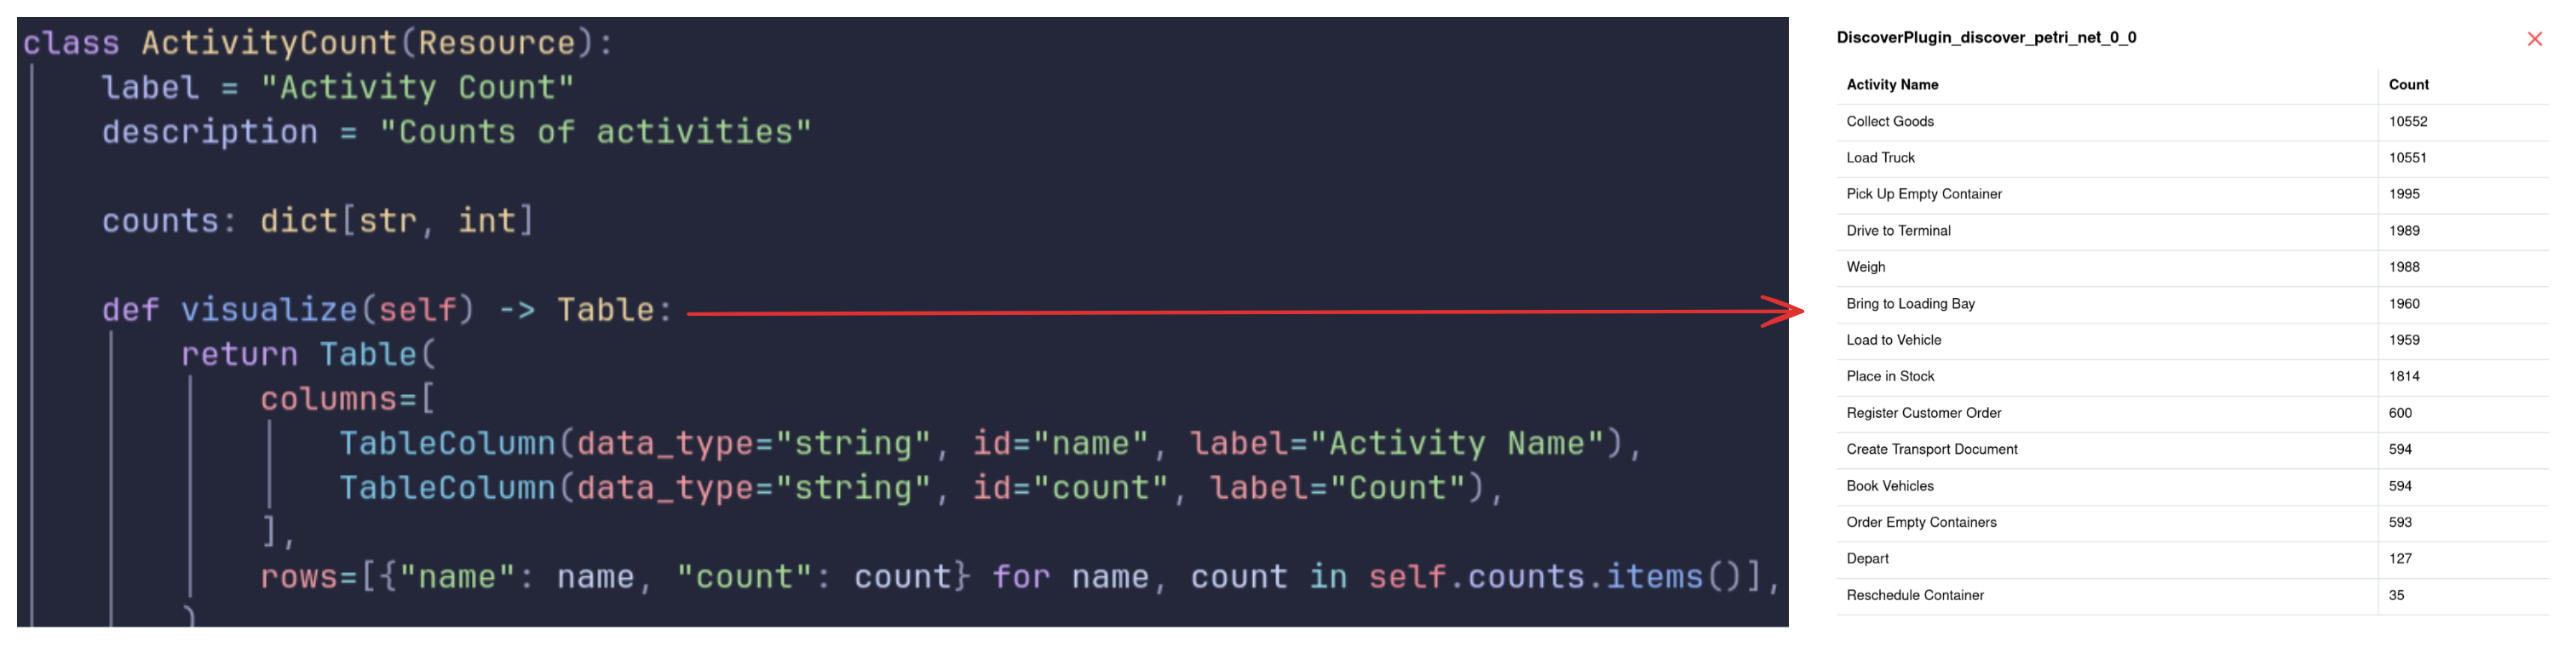
\includegraphics[width=\textwidth]{figures/implementation/ActivityCountResource.png}
	\caption{Example of a resource that returns a \texttt{Table} through its \texttt{visualize()} method, which the frontend renders.
	}
	\label{fig:activity-count-resource}
\end{figure}

\subsection{Plugin Implementation}

Plugins and their plugin functions are implemented by extending the \texttt{Plugin} base class provided by the \textit{Ocelescope} package.
Each plugin defines exactly one plugin class.
Similar to resources, a plugin class declares metadata such as a label, a description, and a version through class attributes.
These values are displayed in the plugin interface in the frontend.

Plugin functions are implemented as class methods.
Each method is marked with a decorator that registers it as a plugin method.
The decorator can also define metadata such as a readable name and a short description, which are shown in the user interface.
This design keeps the declaration of plugin functions simple and consistent, and avoids the need for additional configuration formats or boilerplate code.

\begin{figure}[ht]
	\centering
	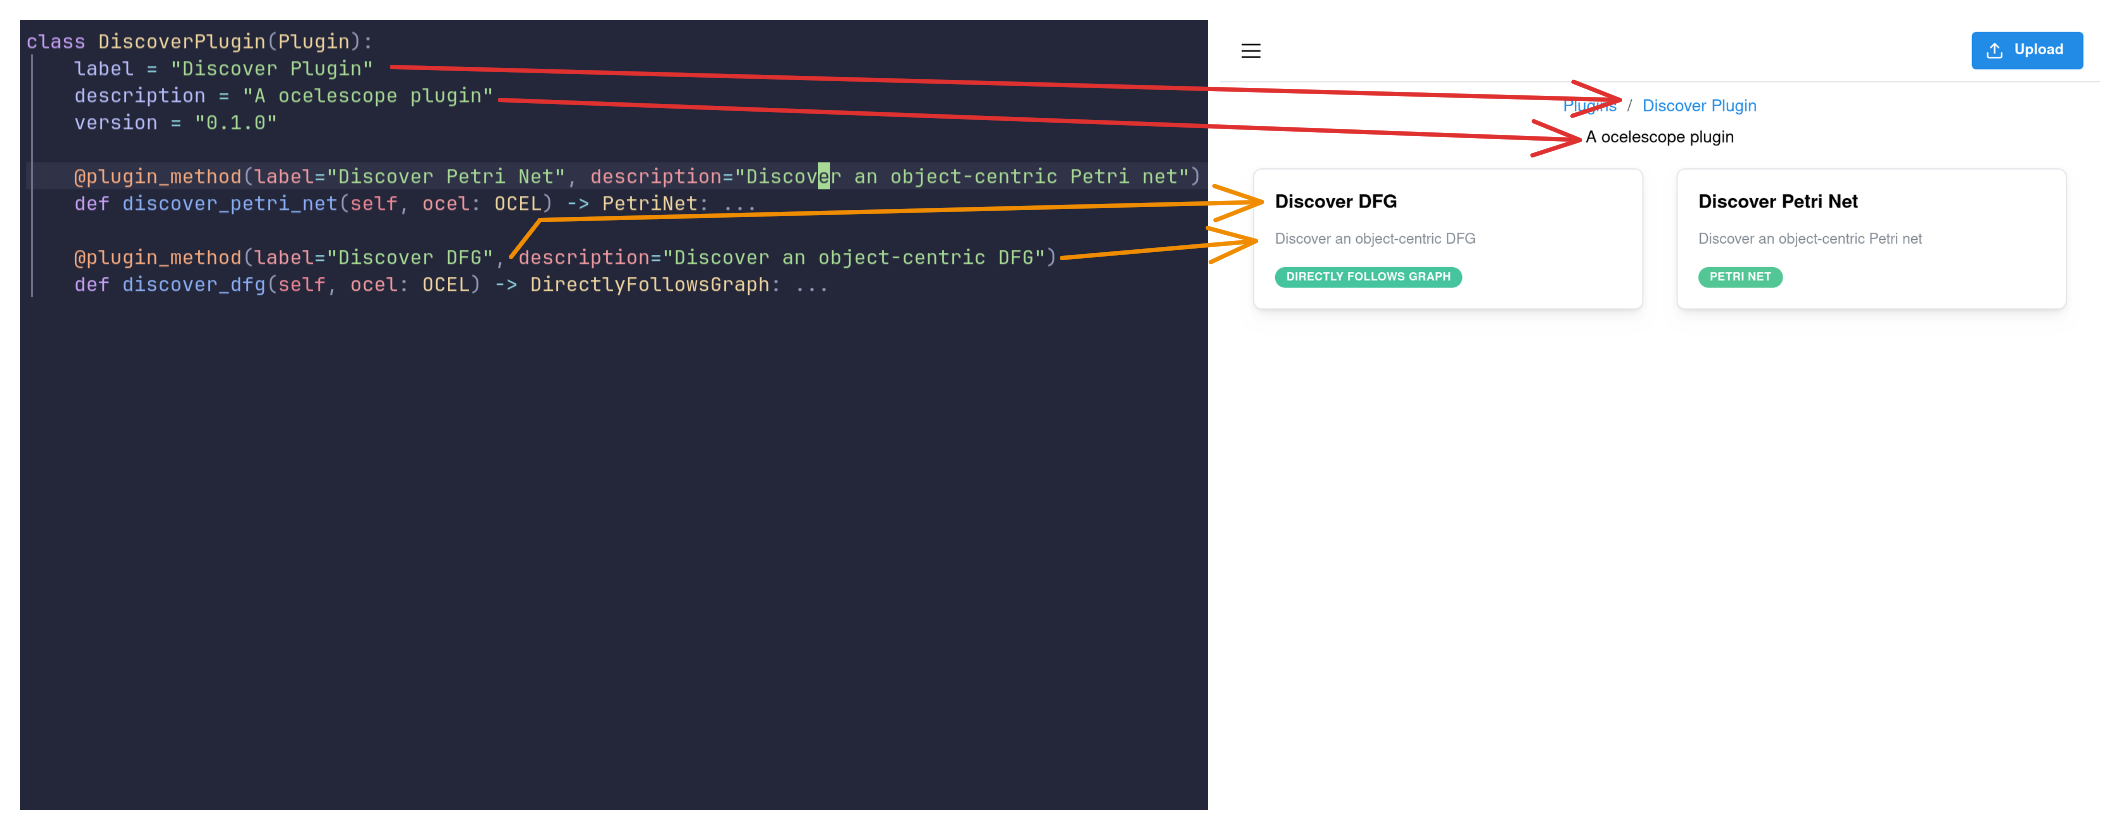
\includegraphics[width=\textwidth]{figures/implementation/plugintouimapping.png}
	\caption{Mapping between a plugin class in Python and its representation in the frontend.
		Class metadata defines the plugin entry, and each decorated method appears as a callable function with its own label and description.}
	\label{fig:plugin-to-ui-mapping}
\end{figure}

\paragraph{Generation of Input Interfaces}

The input of a plugin function is automatically derived from its function signature.
OCEL and resource parameters are inferred directly from the plugin method and rendered as selectable entries in the form.

Configuration inputs are defined as Python classes that inherit from Pydantic base classes.
This allows them to be validated automatically and converted into JSON Schema.
Helper functions can be used to add metadata such as titles, descriptions, default values, or field restrictions, which are reflected in the generated frontend form.

OCEL-dependent fields are defined using helper functions similar to those in Pydantic.
They specify the type of OCEL-dependent field and reference a specific OCEL parameter by name.
When the user selects an OCEL, the frontend requests the required information from the backend and populates the field automatically, for example with event types or object types.

Dynamic configuration fields are also defined through helper functions.
Instead of referencing an OCEL parameter, they reference functions defined inside the input class.
These functions receive the current partial form state.
Whenever the form changes, the backend evaluates them.
If they return a value, the corresponding field is updated.
This makes it possible to compute input options dynamically based on earlier user selections.

\begin{figure}[ht]
	\centering
	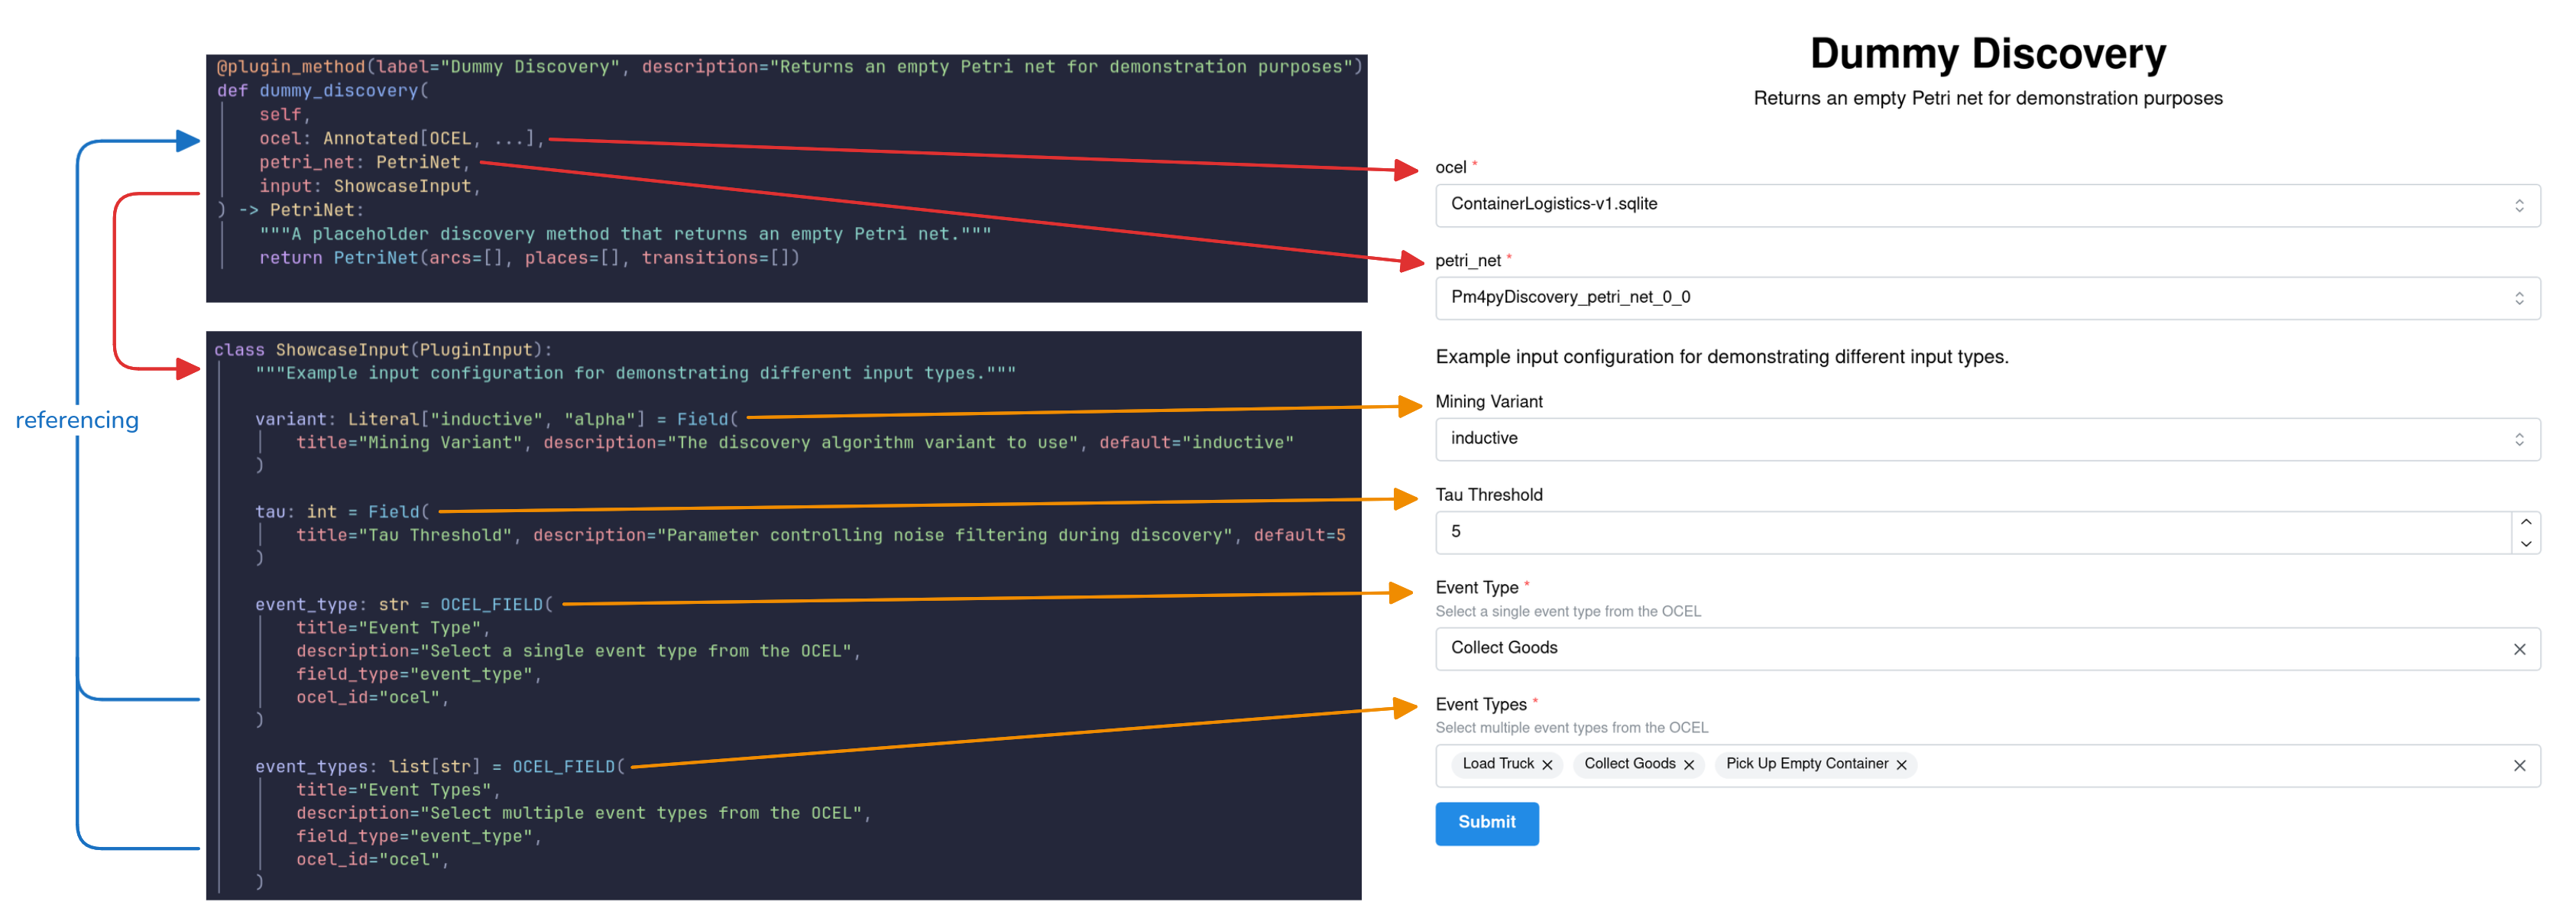
\includegraphics[width=\textwidth]{figures/implementation/DummyDiscovery.png}
	\caption{Plugin method parameters and their corresponding auto-generated input form.
		OCEL and resource parameters appear as selection fields, while configuration parameters are derived from Pydantic-based input classes.}
	\label{fig:dummy-discovery-input}
\end{figure}

\paragraph{Rust support through Python bindings.}
Plugin functions in \textit{Ocelescope} are executed as Python code in the backend.
At the same time, Requirement \req{EX-6} specifies that process mining functionality can be implemented in Python or Rust.
In the current implementation, Rust support is therefore provided as a pragmatic compromise through Python bindings, as shown in~\cite{rust4pm}.
This makes it possible to use Rust-based functionality from within Python plugins.
In \textit{Ocelescope}, Rust code can be exposed to Python, packaged as a Python wheel, and bundled with a plugin archive.
When the plugin is loaded, the wheel can be used like a regular Python dependency, which allows plugin functions to call Rust-based functionality through the Python interface.

\section{Module Implementation}

Modules are implemented in a way that stays close to common frontend and backend development practices. A frontend module behaves like a normal React application. A backend module behaves like a normal Python router. The only additional concept is the way modules are embedded into \textit{Ocelescope}.

\subsection{Frontend Modules}

Frontend modules are defined through a small configuration written in TypeScript. The configuration specifies the name of the module and its metadata. A module also provides one or more routes. Each route implements a view and is written as a normal React component.

During the build step, the module folders are scanned through static analysis. All pages found inside a module are added to the internal router of the application. Each page is compiled and rendered inside the shared application shell. The module pages are also added to the sidebar so that they can be accessed in the same way as the built-in views.

\begin{figure}[h]
	\centering
	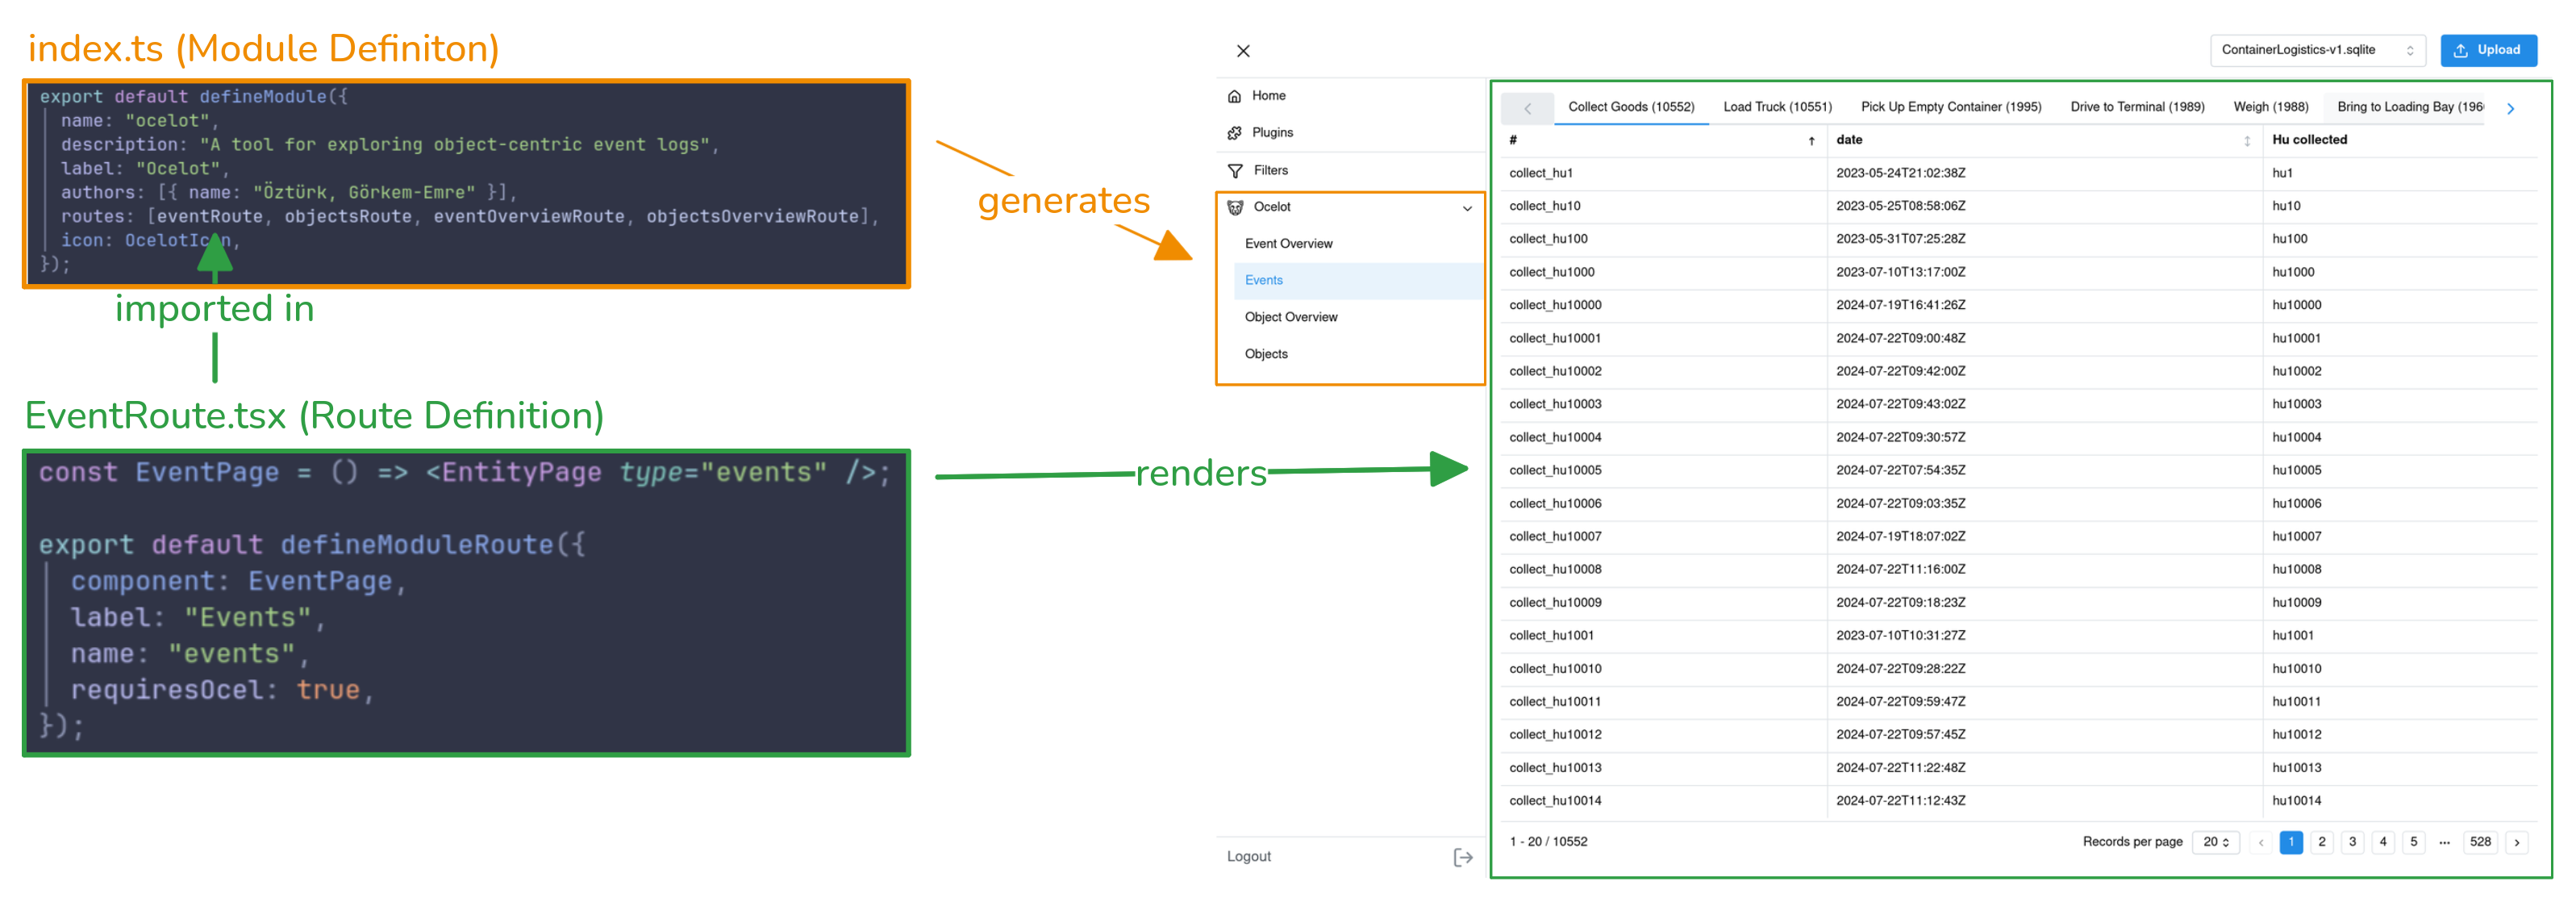
\includegraphics[width=\textwidth]{./figures/implementation/frontendmoduleimpl.png}
	\caption{Frontend modules inside \textit{Ocelescope}. The application shell integrates each module and provides navigation.}
	\label{fig:frontend_modules}
\end{figure}

\subsection{Backend Modules}

Backend modules are implemented as Python modules that are stored inside a dedicated modules folder. When \textit{Ocelescope} starts, these modules are imported dynamically. Each backend module defines a FastAPI subrouter. This subrouter is attached to the main API router and all endpoints of the module appear under a shared prefix.

Backend modules can access OCELs and session data through dependency injection. A module can also define its own internal state. The state is implemented as a simple Python class. It is stored inside the session and is created and persisted automatically.

\begin{figure}[h]
	\centering
	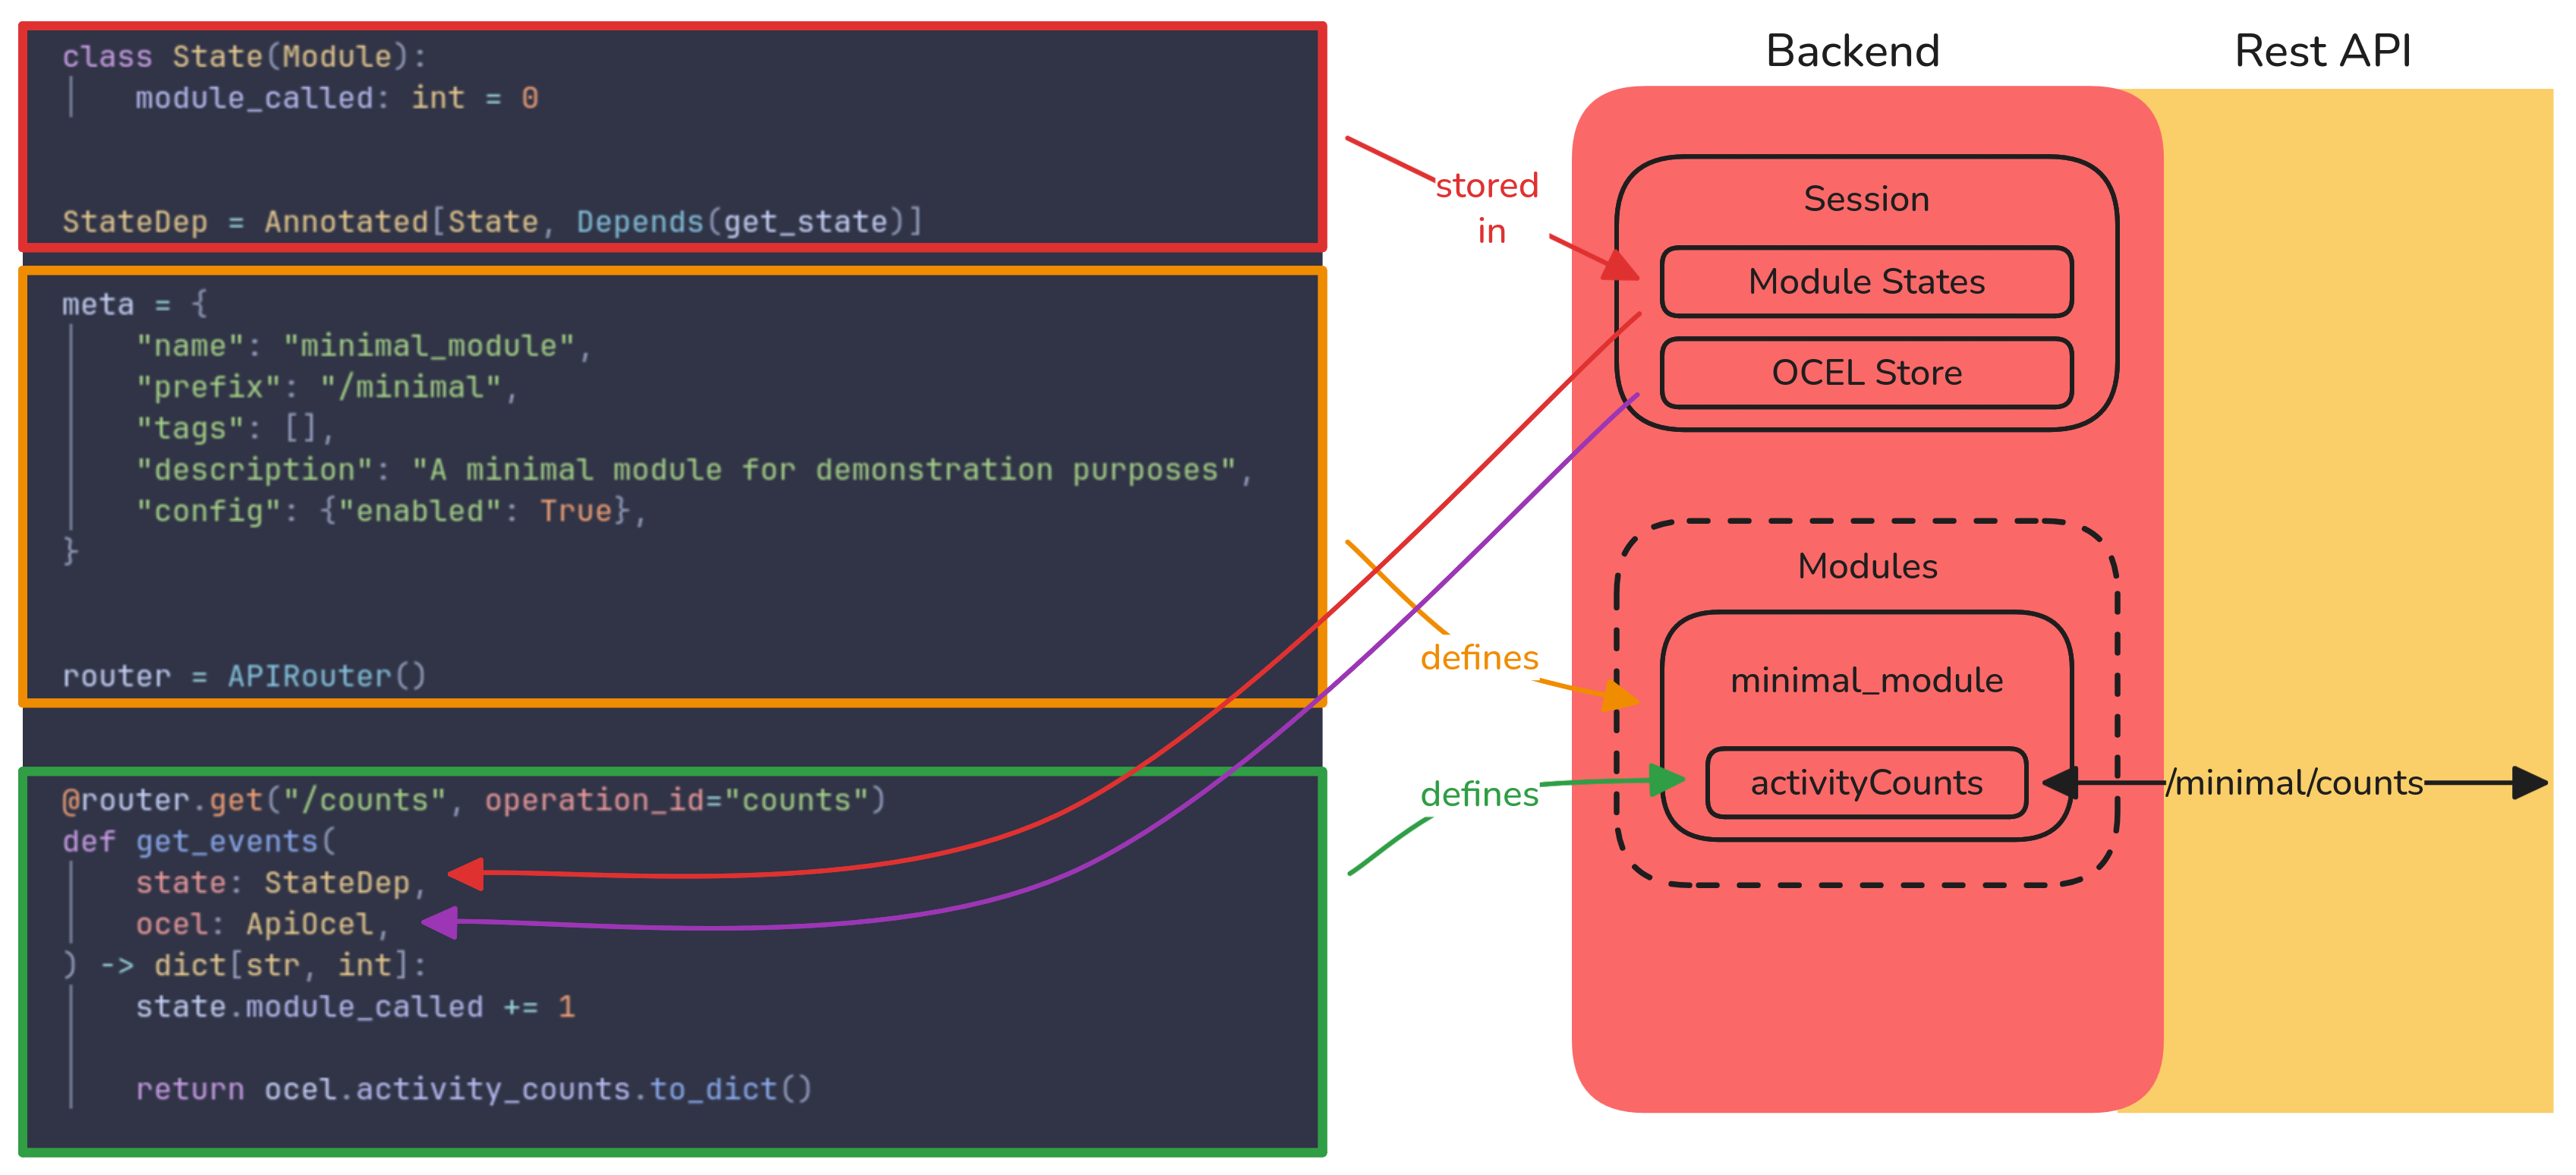
\includegraphics[width=0.8\textwidth]{./figures/implementation/BackendModuleImplementation.png}
	\caption{Structure of a backend module. The module defines metadata, a router, and a state object. The state is stored inside the session and is available through dependency injection.}
	\label{fig:backend_module}
\end{figure}

\subsection{Standard Functionality Implemented as Modules}

Basic functionality such as filtering and inspection is implemented through modules. The inspection module is based on the design of Ocelot and provides tables and summaries of events and objects. The filter module implements the standard filters of the Ocelescope package and allows users to apply them through a graphical interface.

\paragraph{Filtering}
Each OCEL in a session has a filter pipeline that stores the active filters. The filter view provides a graphical interface for all predefined filters of the Ocelescope package. The filters do not create new OCEL instances. They only update the current filter state of the selected log.

\begin{figure}[h]
	\centering
	\begin{subfigure}{0.48\textwidth}
		\centering
		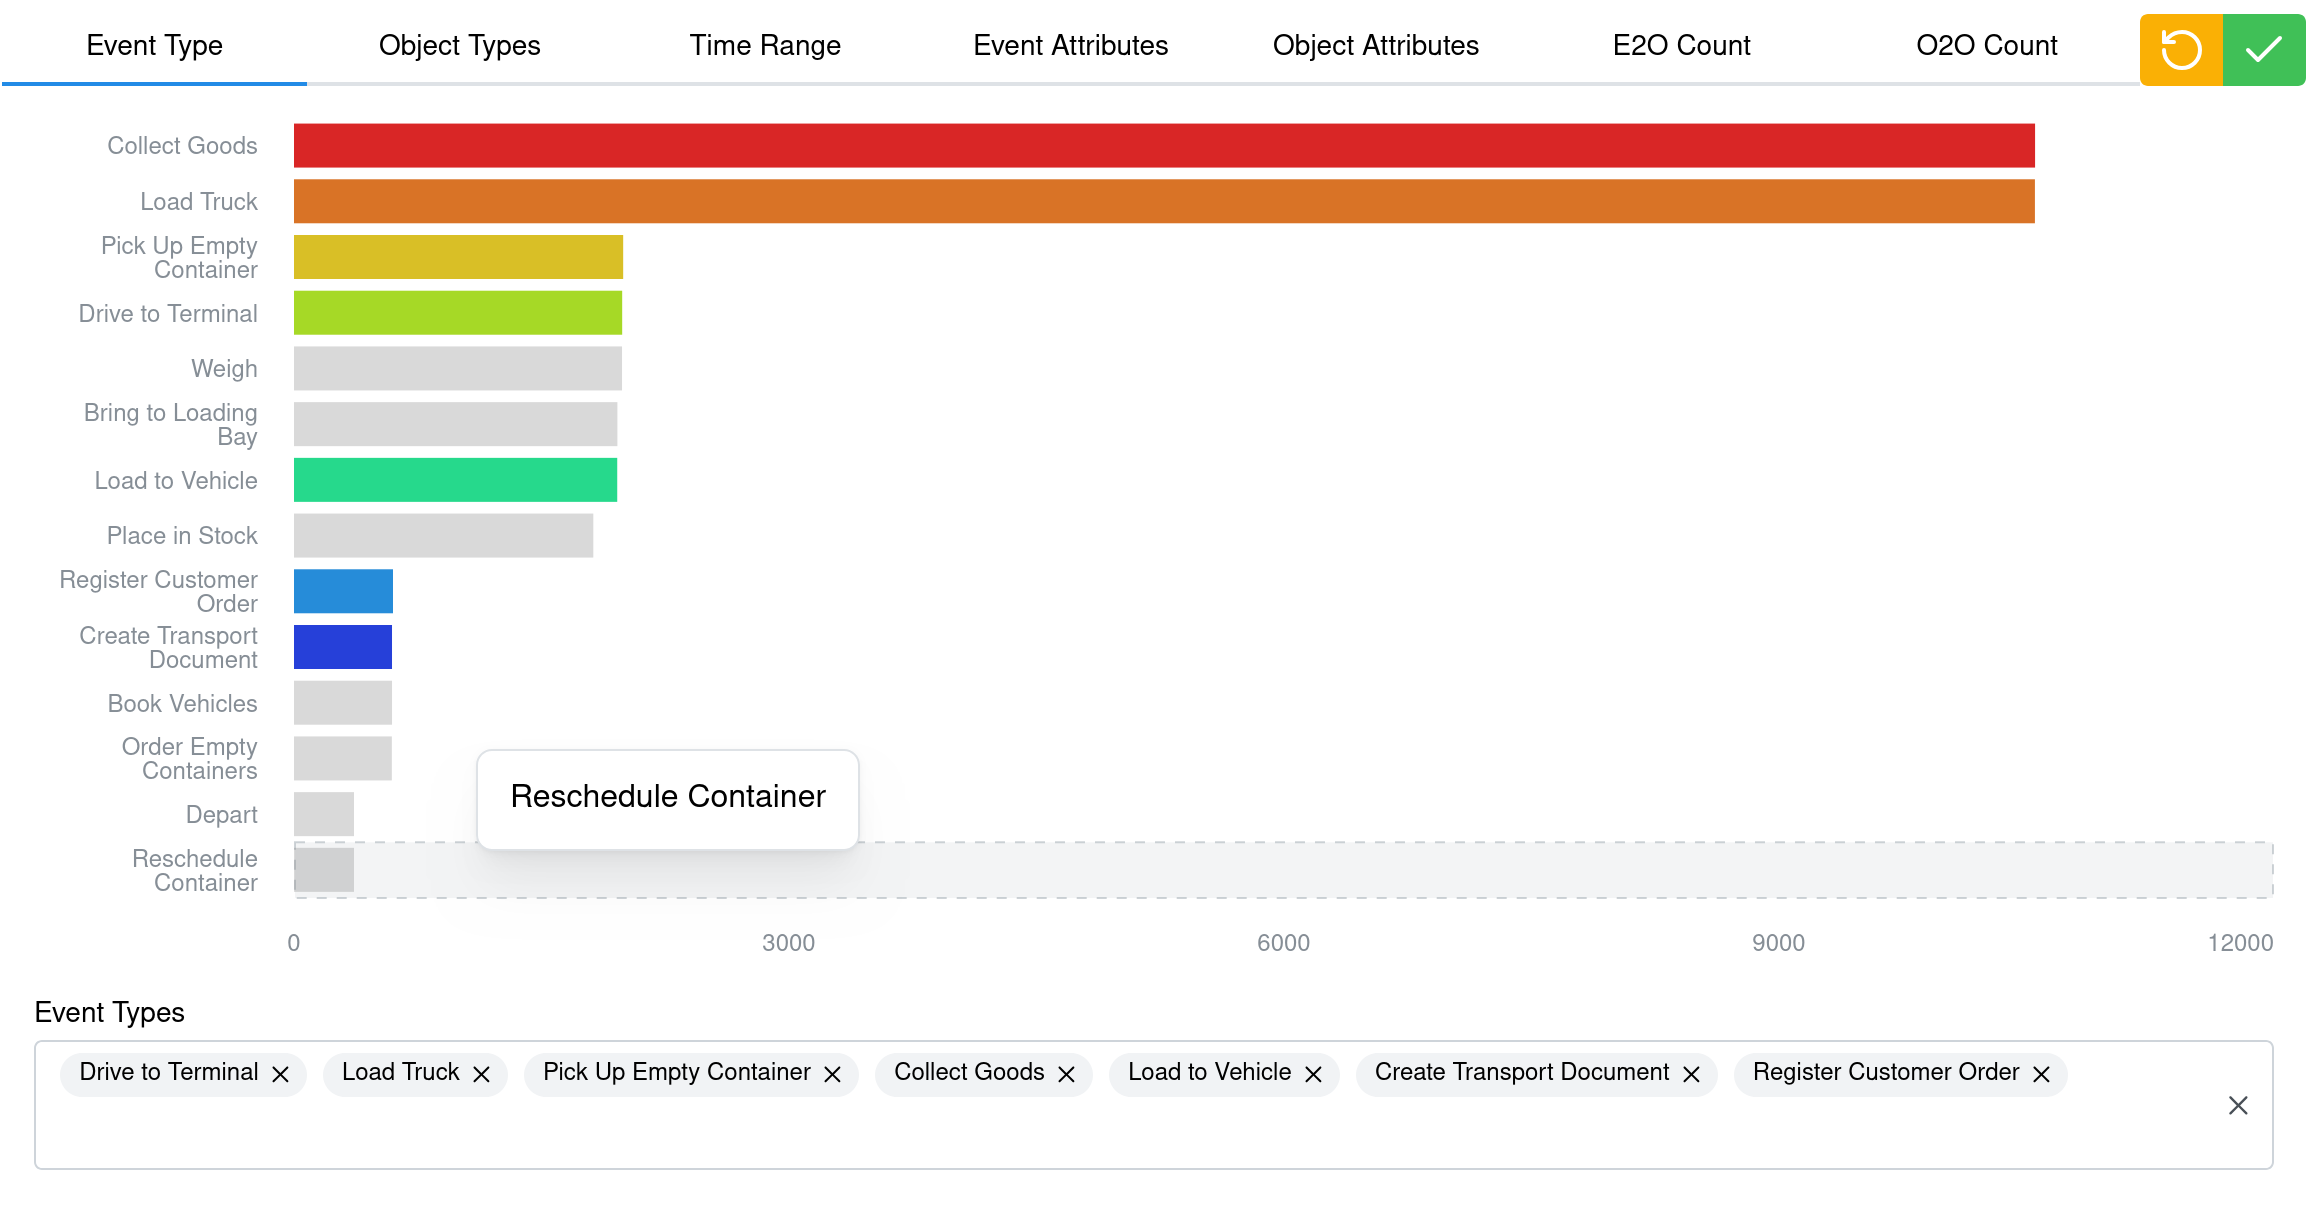
\includegraphics[width=\textwidth]{./figures/implementation/activitycountfilter.png}
		\caption{Activity filter}
	\end{subfigure}
	\hfill
	\begin{subfigure}{0.48\textwidth}
		\centering
		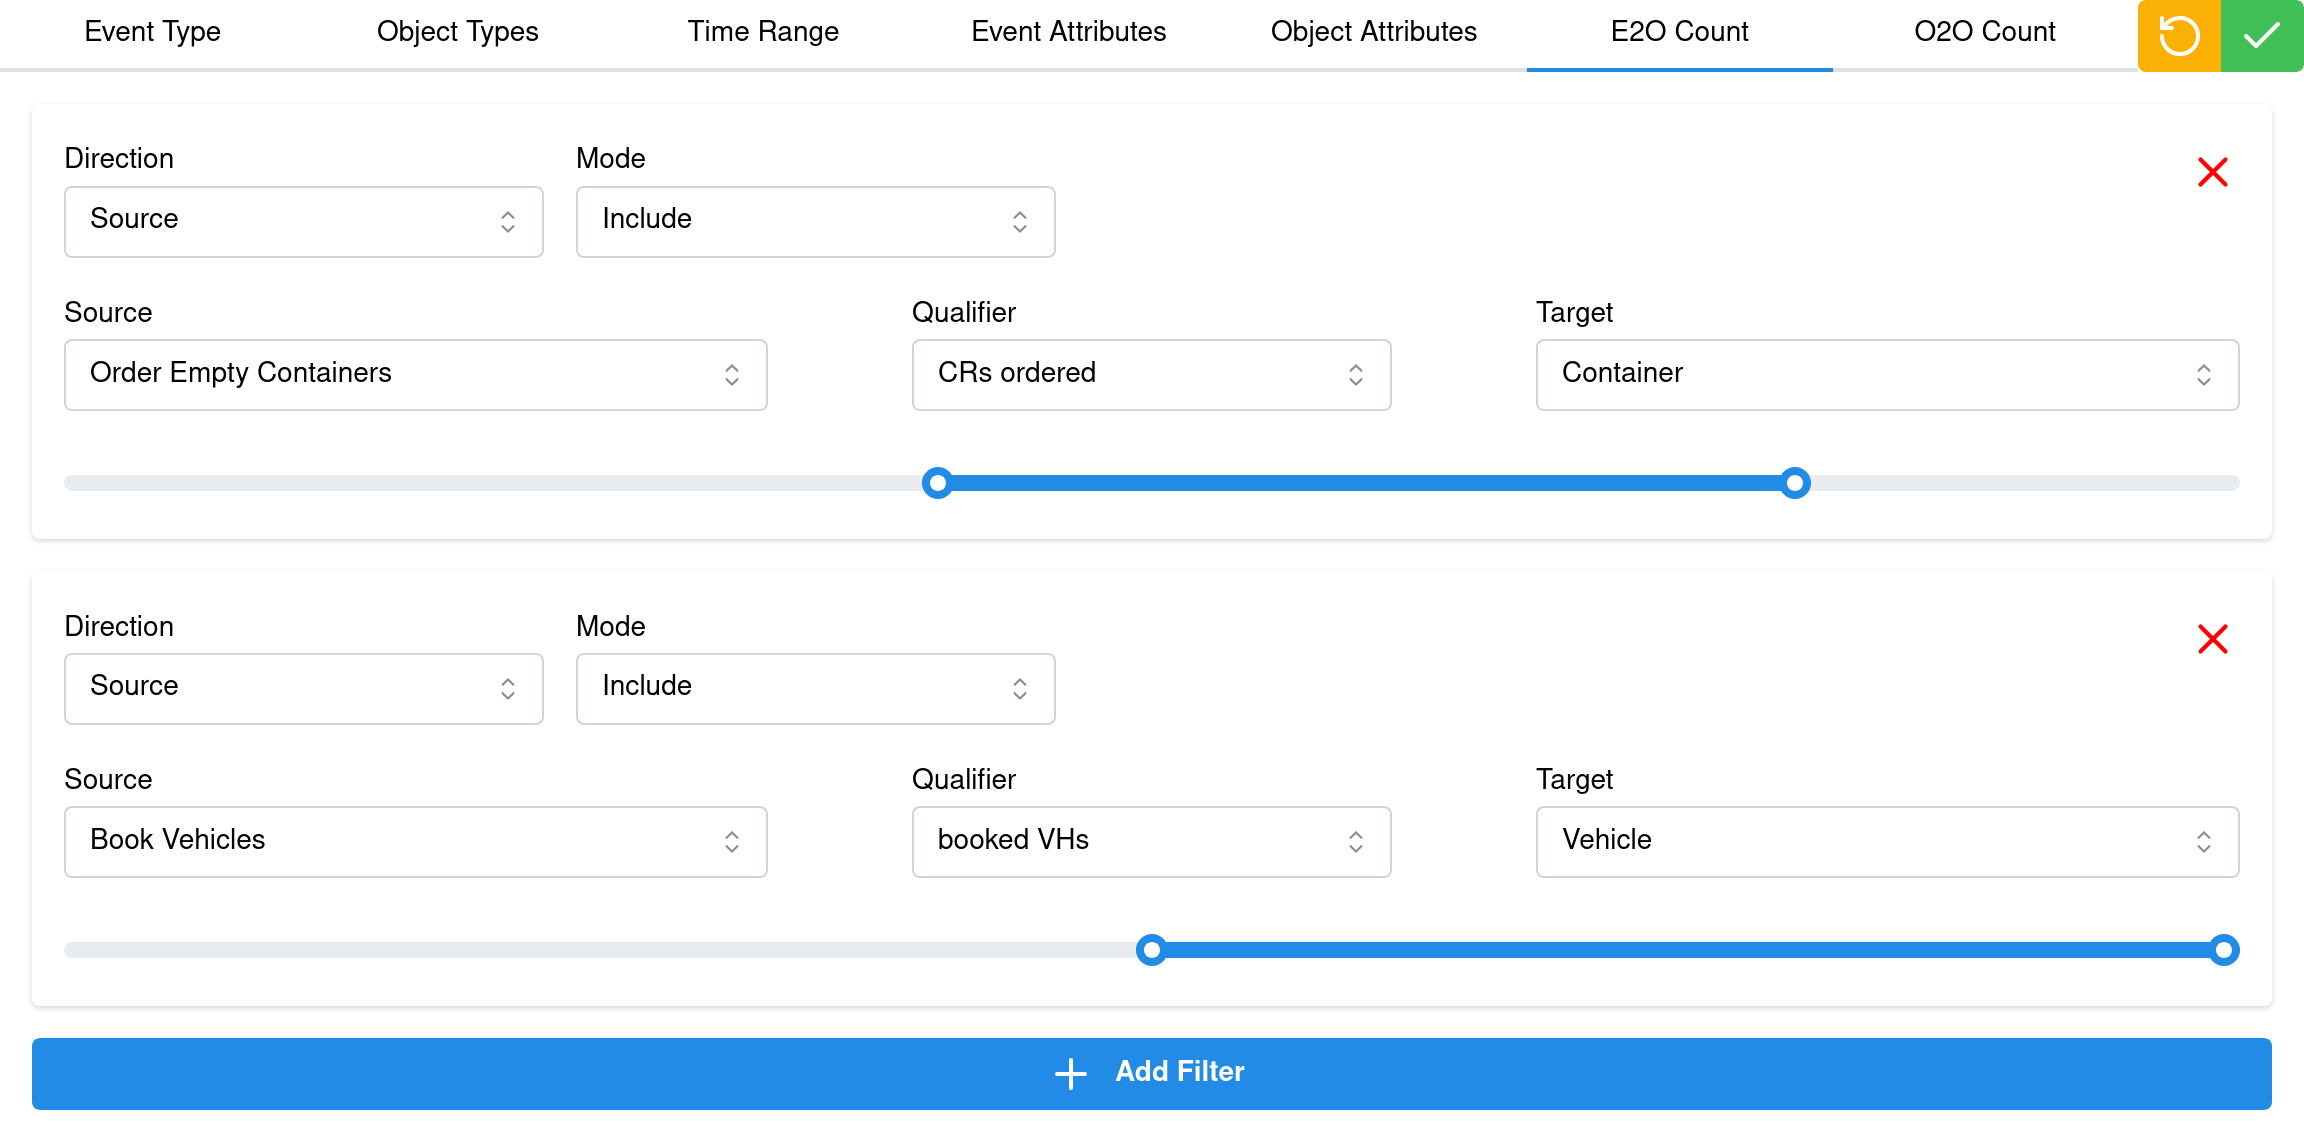
\includegraphics[width=\textwidth]{./figures/implementation/relationfilter.png}
		\caption{E2O count filter}
	\end{subfigure}
	\vspace{0.3cm}
	\begin{subfigure}{0.48\textwidth}
		\centering
		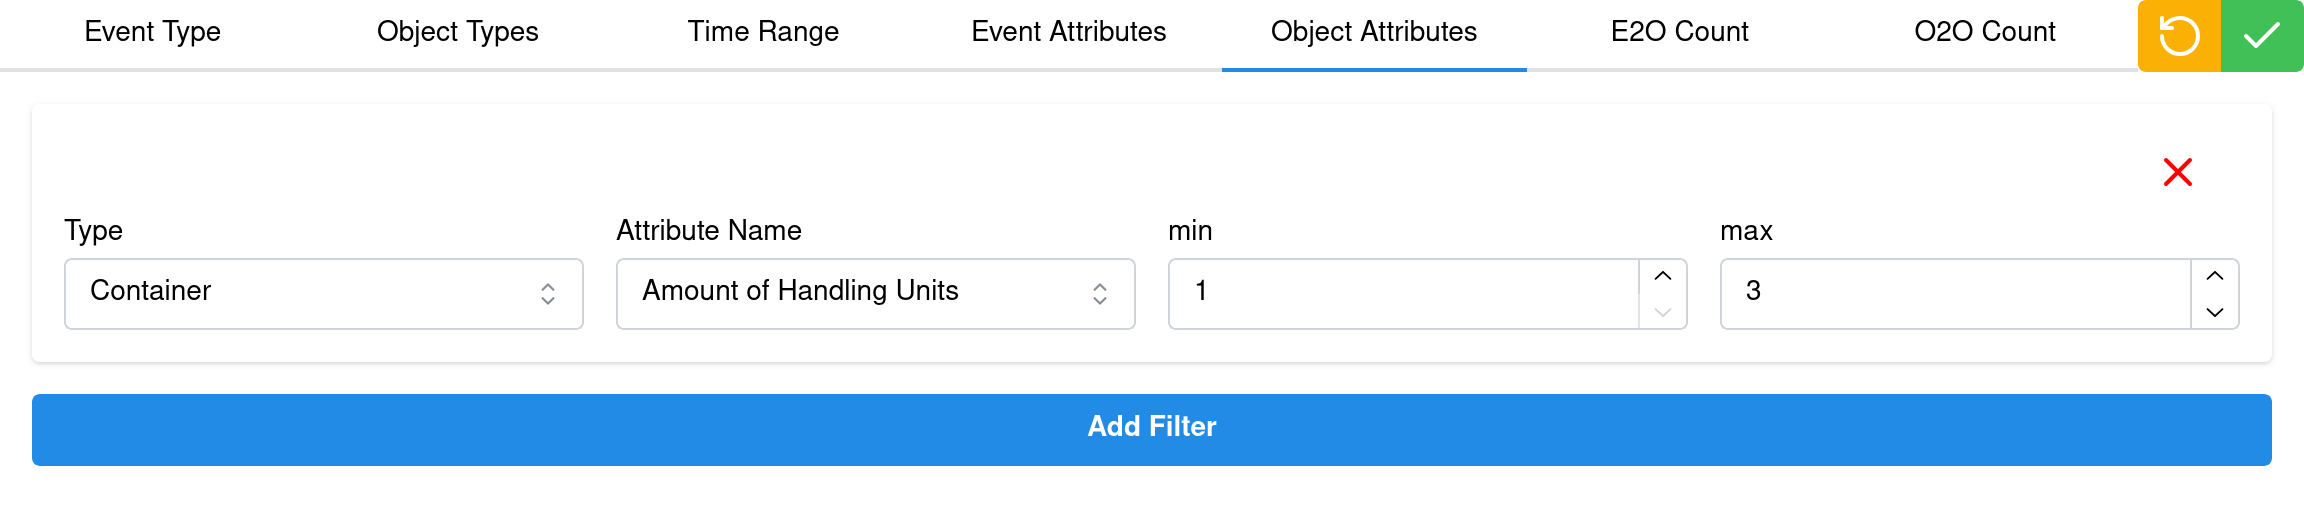
\includegraphics[width=\textwidth]{./figures/implementation/oattrifilter.png}
		\caption{Object attribute filter}
	\end{subfigure}
	\hfill
	\begin{subfigure}{0.48\textwidth}
		\centering
		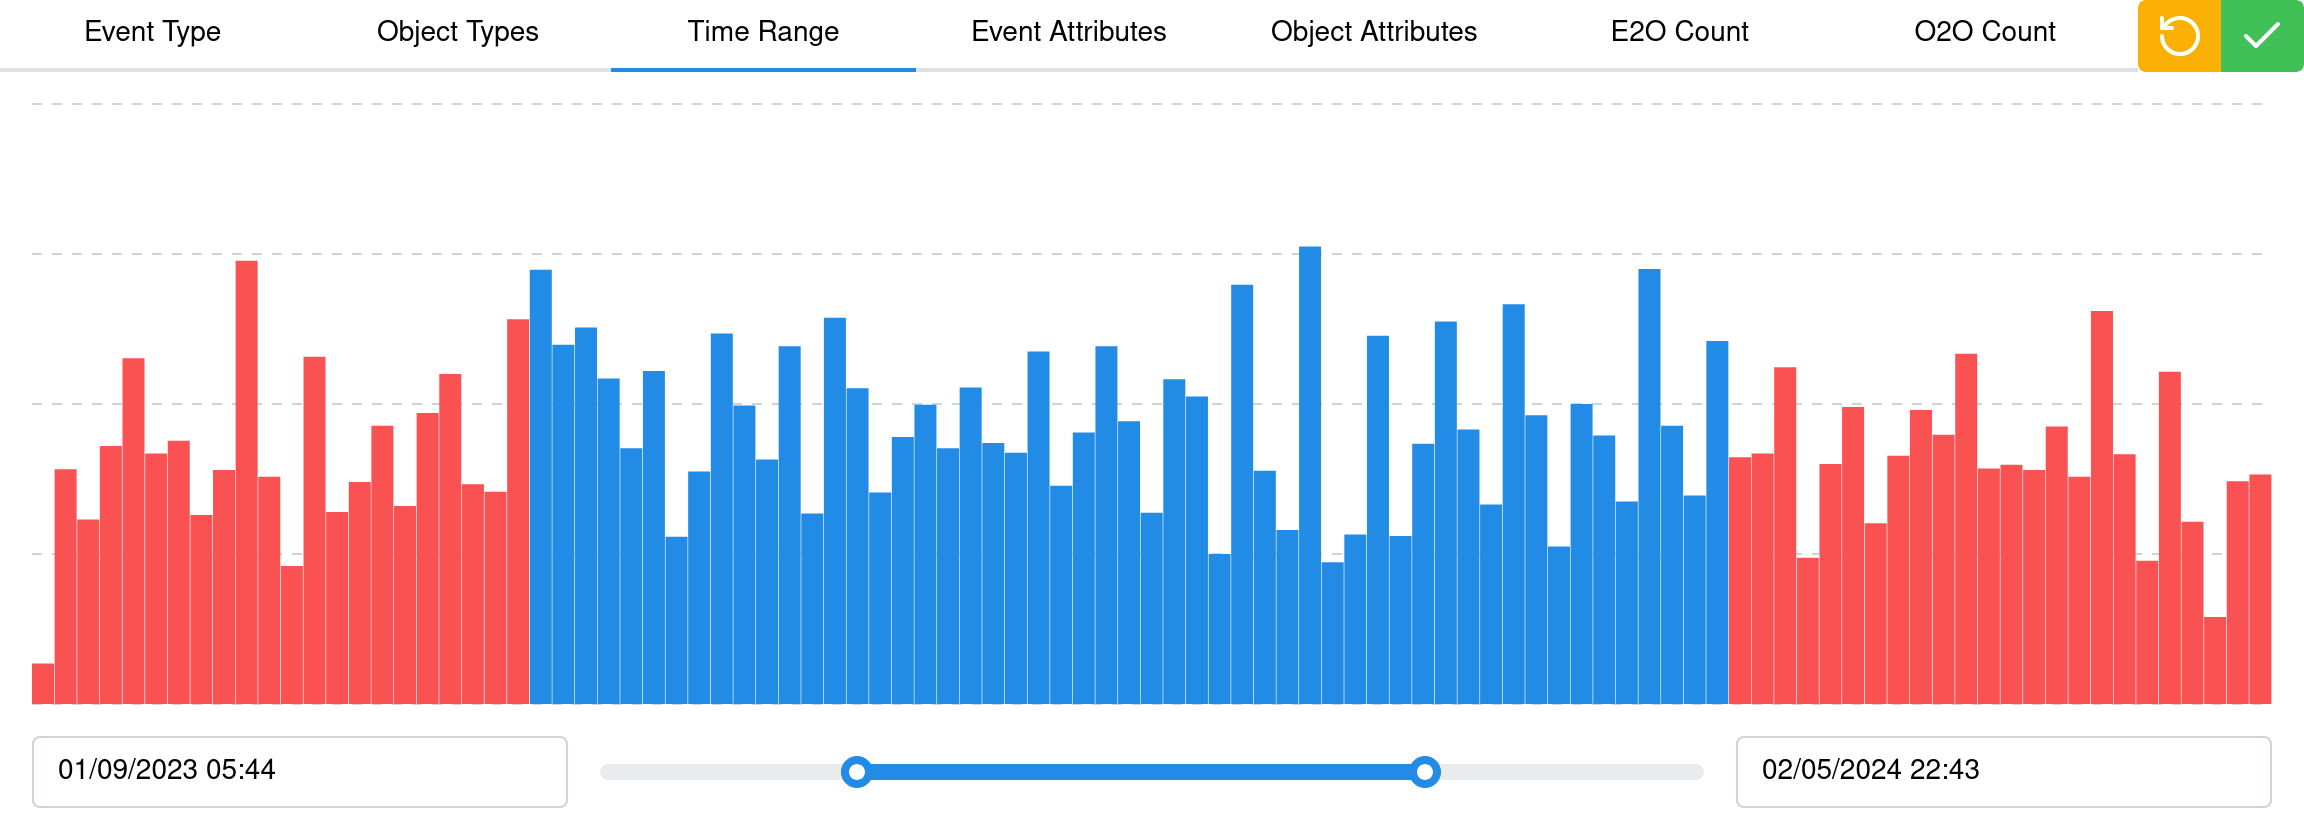
\includegraphics[width=\textwidth]{./figures/implementation/timeframefilter.png}
		\caption{Time range filter}
	\end{subfigure}

	\caption{Overview of the filter types available in Ocelescope.}
	\label{fig:filters_overview}
\end{figure}

\paragraph{OCEL Inspection}

OCEL inspection provides an interface for exploring the structure and contents of a log. It offers four views that give access to events, objects, and their relations:

\begin{itemize}
	\item \textbf{Objects View:} A table of all objects with their attributes and related entities.
	\item \textbf{Events View:} A table of events with their attributes and linked objects.
	\item \textbf{Object Summary:} A compact overview of object attributes and relations, including visual representations.
	\item \textbf{Event Summary:} A similar overview for events, showing attribute distributions and relation patterns.
\end{itemize}

Inspection uses cached information to keep navigation responsive even for larger logs.

\begin{figure}[h]
	\centering
	\begin{subfigure}{0.32\textwidth}
		\centering
		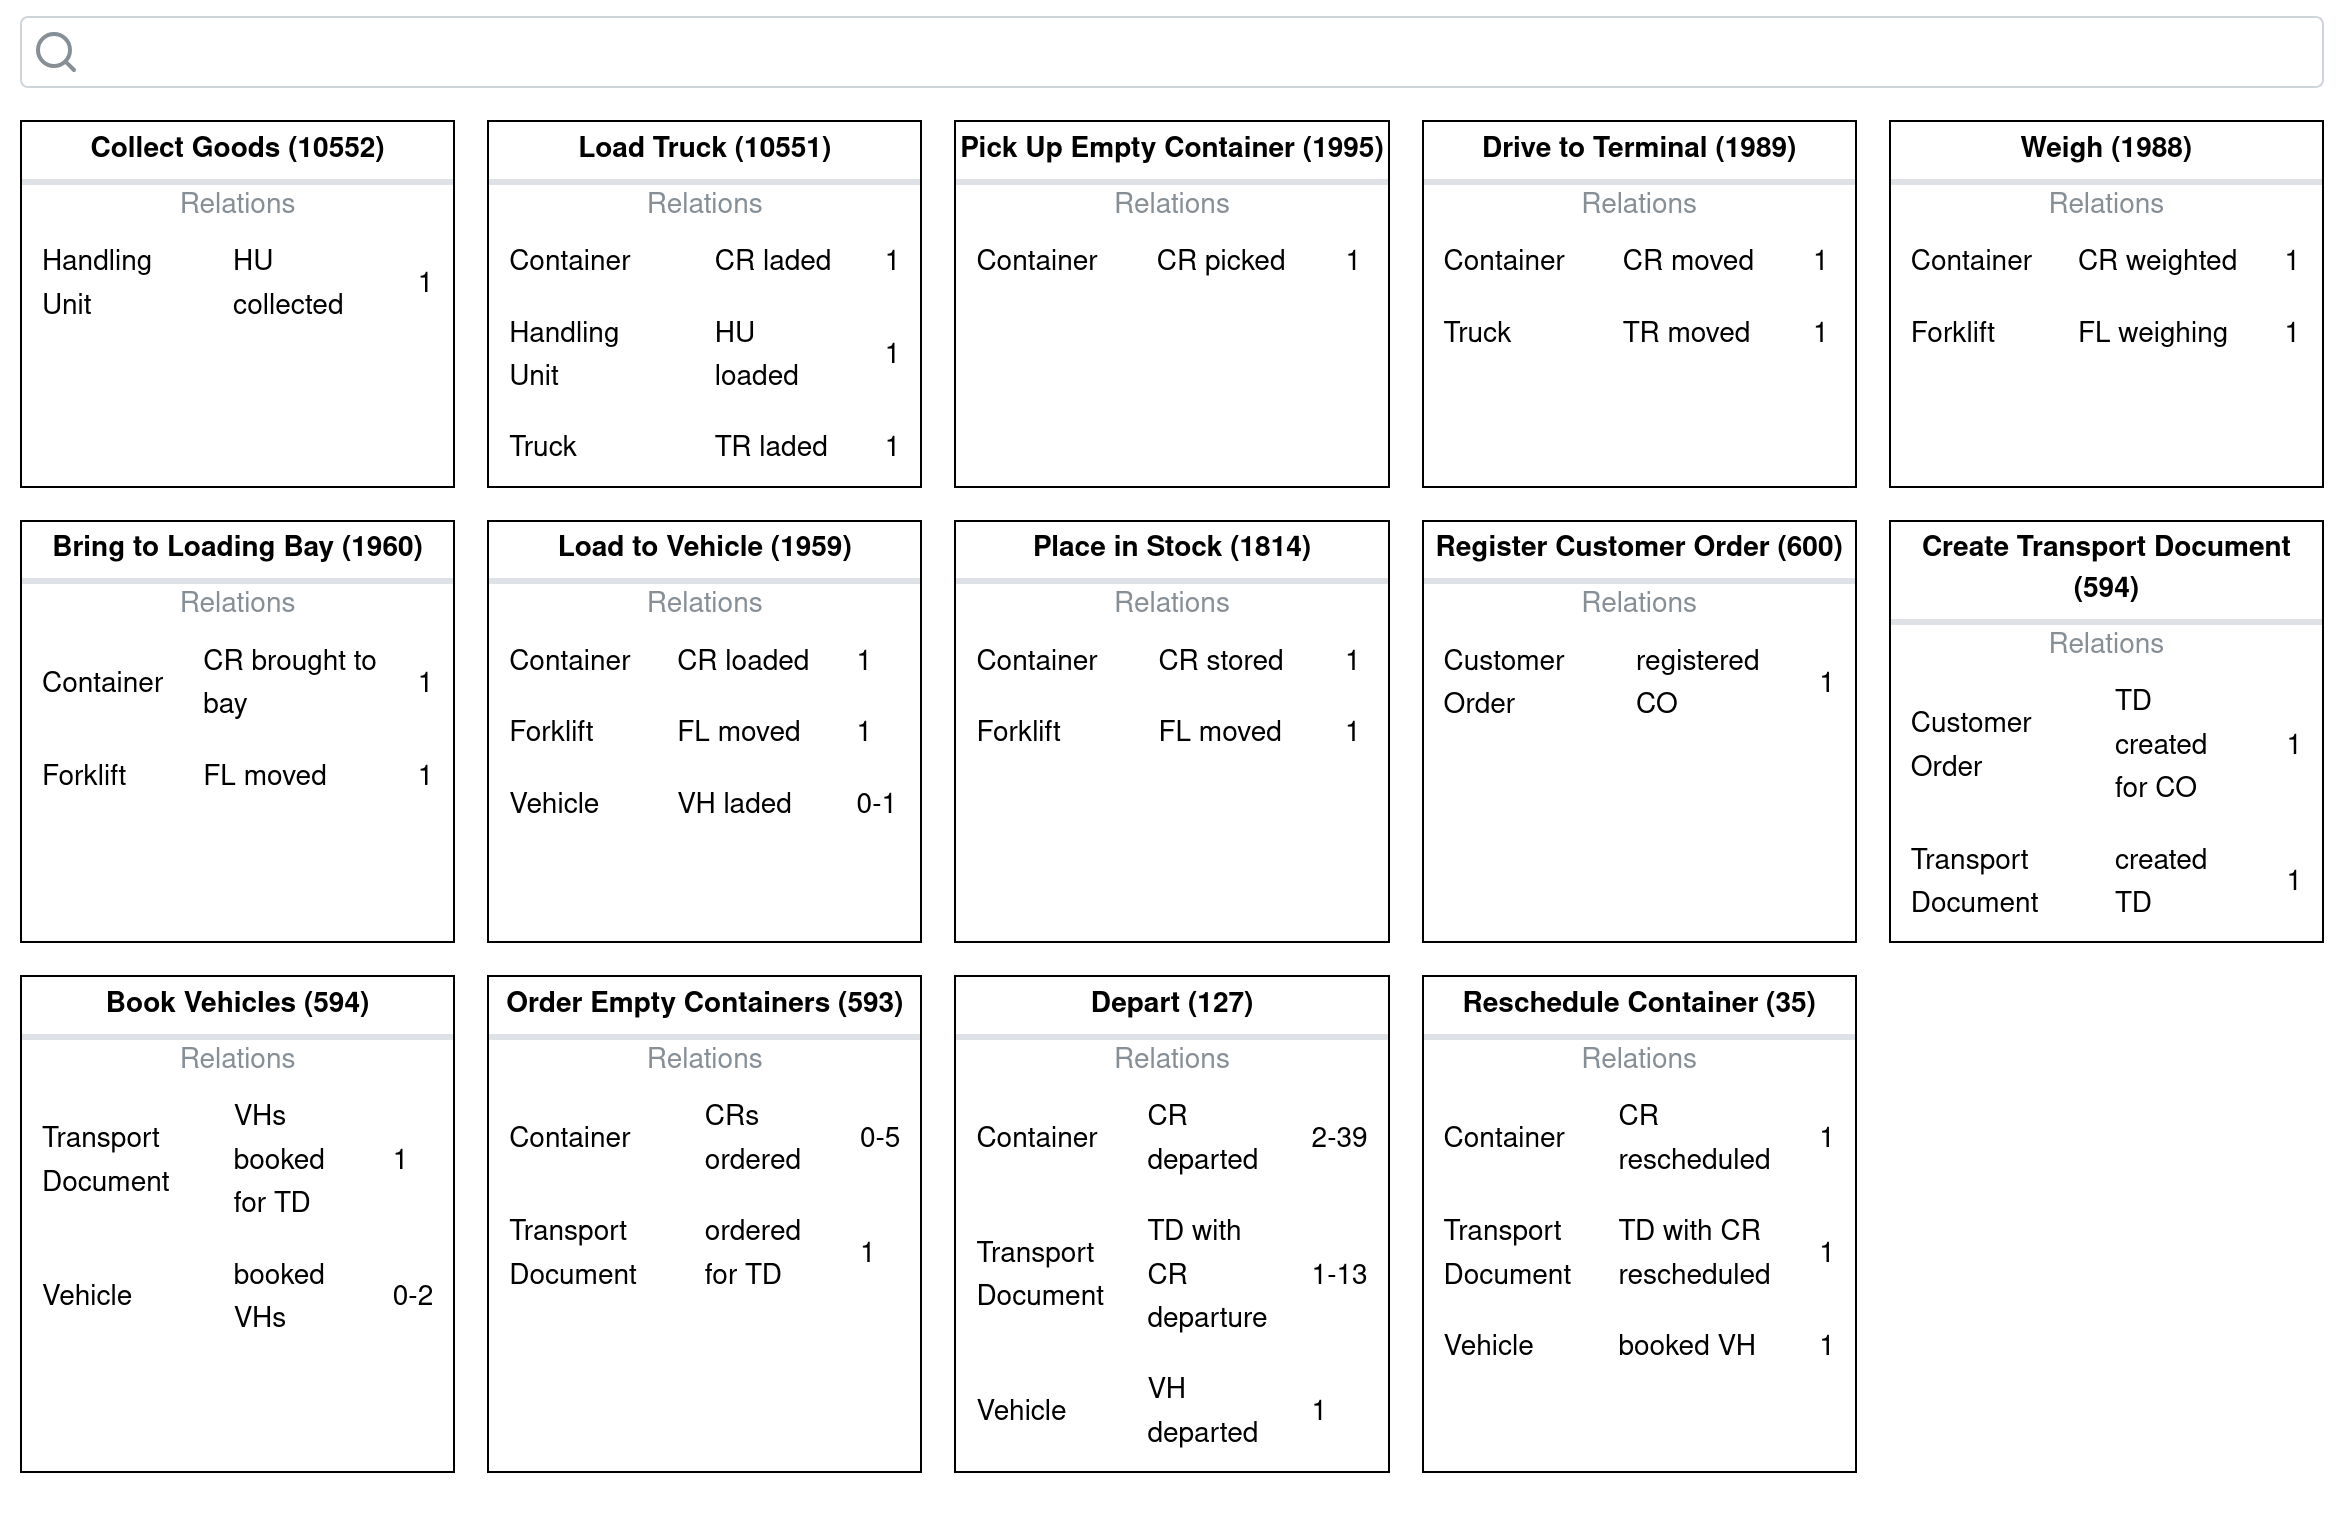
\includegraphics[width=\textwidth]{./figures/implementation/eventoverview.png}
		\caption{Events view}
	\end{subfigure}
	\hfill
	\begin{subfigure}{0.32\textwidth}
		\centering
		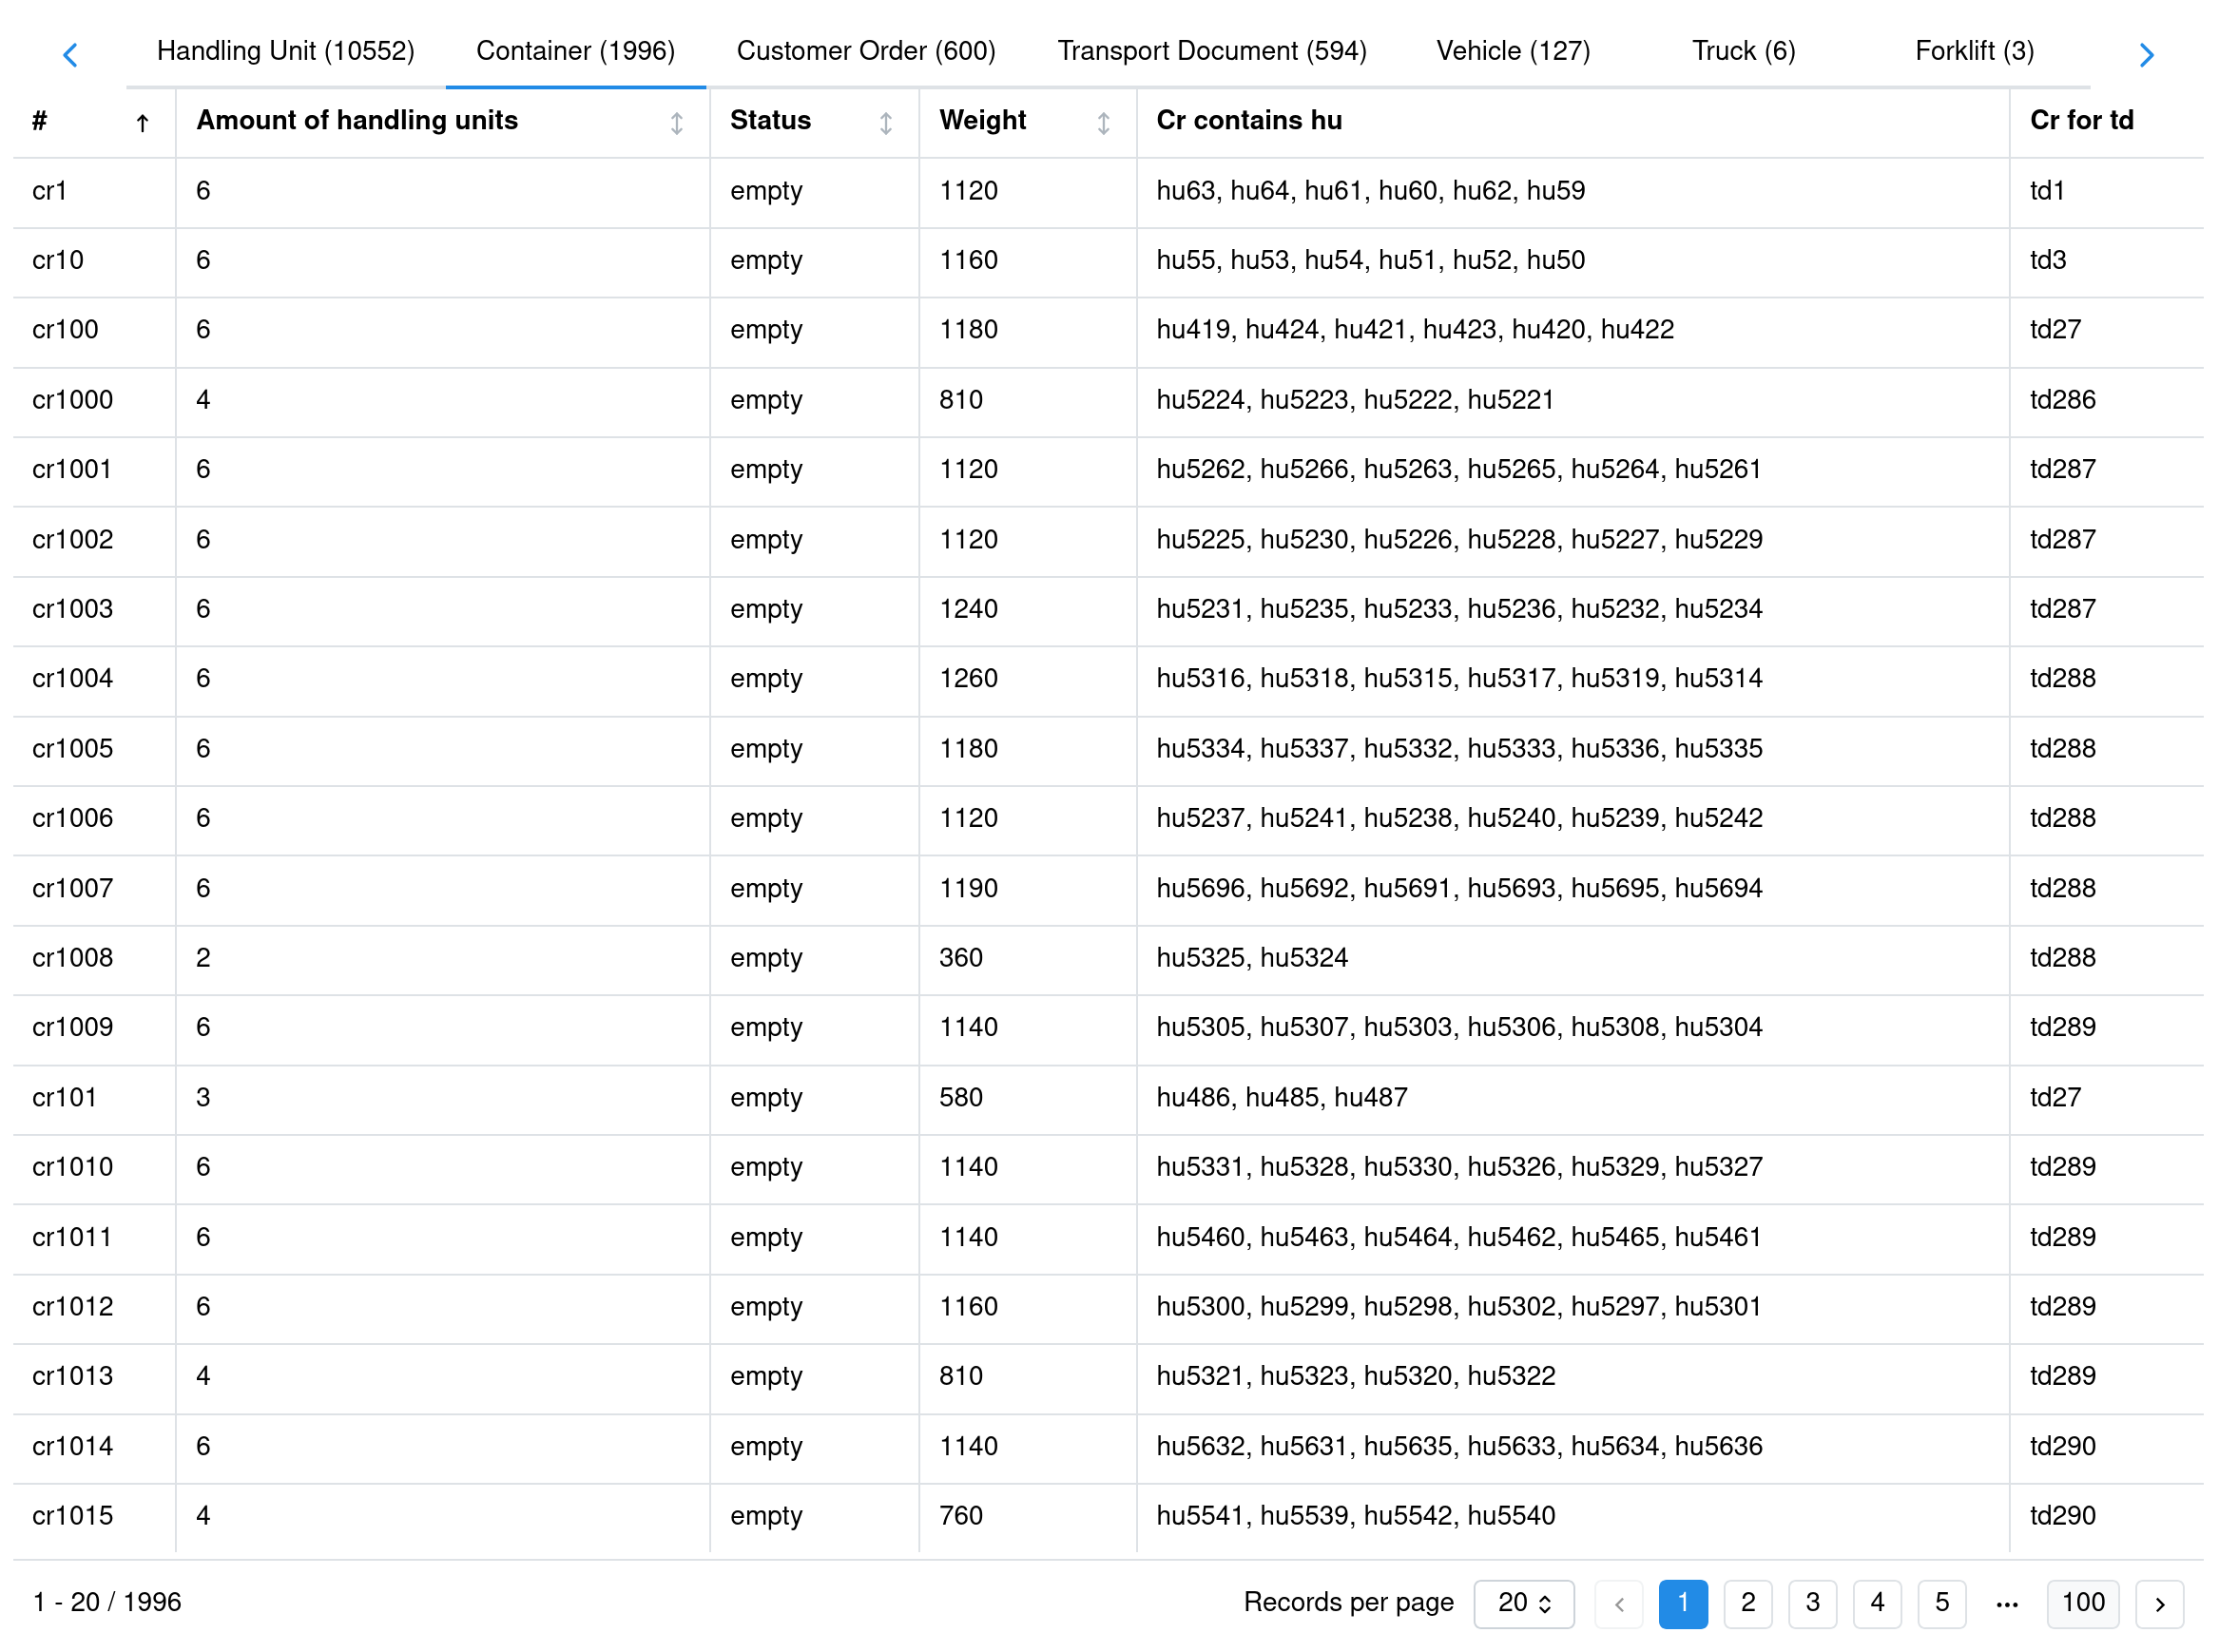
\includegraphics[width=\textwidth]{./figures/implementation/objectentities.png}
		\caption{Objects view}
	\end{subfigure}
	\hfill
	\begin{subfigure}{0.32\textwidth}
		\centering
		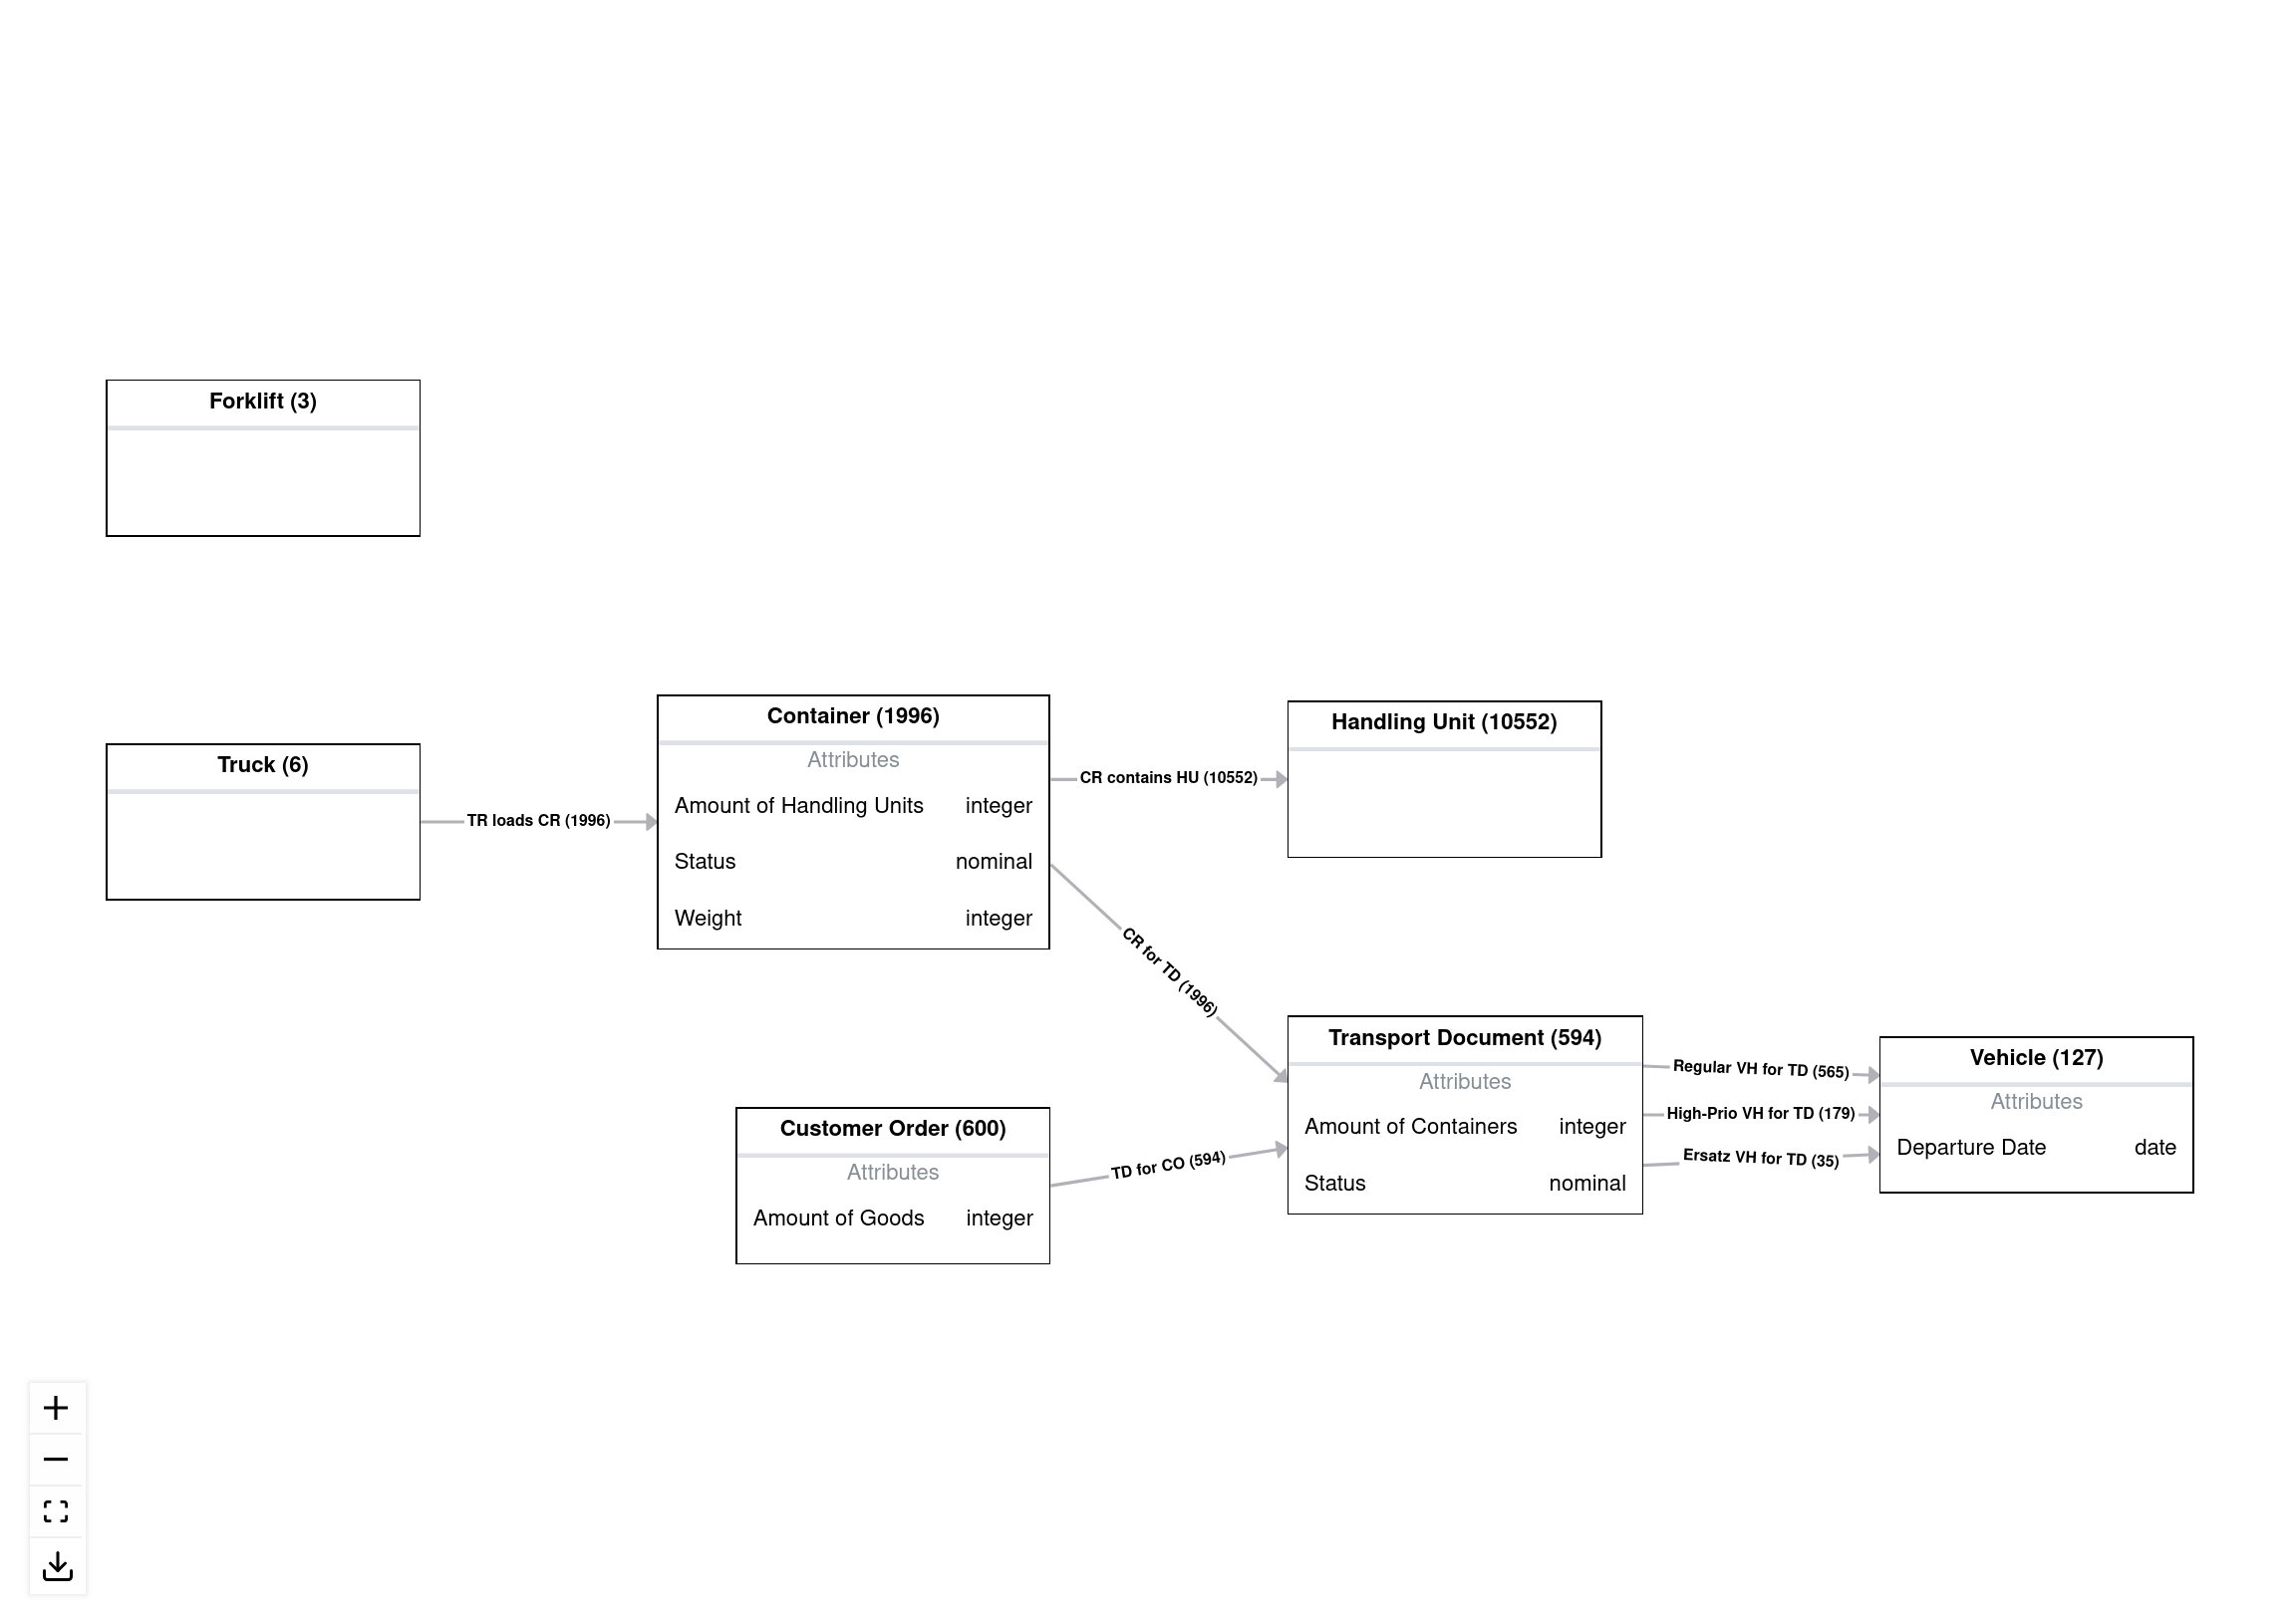
\includegraphics[width=\textwidth]{./figures/implementation/objectoverview.png}
		\caption{Object summary}
	\end{subfigure}

	\caption{Inspection views.}
	\label{fig:inspection_views}
\end{figure}

\subsection{Documentation}

To support the development of extensions, \textit{Ocelescope} includes a documentation website hosted on GitHub Pages at \url{https://www.ocelescope.org}.
The site is built with MkDocs Material, which was chosen for its simplicity and clear structure, and it is organized into the following parts.

\paragraph{Installation Instructions}
The installation section provides a short setup guide.
Since Docker is the only system requirement, it links to a Docker installation guide.
It then introduces a start command together with a Docker Compose configuration that references the latest frontend and backend images from the container registry.

\paragraph{Plugin Development Guide}
The plugin development guide introduces the core concepts of plugin development.
Each plugin component is presented with an explanation and concrete examples, including common edge cases.
For instance, it explains how to define OCEL-dependent fields and how to restrict configuration fields using Pydantic helper functions.
The guide is intended to make the additional concepts introduced by \textit{Ocelescope} easier to adopt.
Since the documentation is built with MkDocs, it also supports full-text search and can therefore be used as a lookup reference during development.
It also includes a tutorial that implements a more complex plugin with nested input fields and a \texttt{Graph} visualization.
In addition, the tutorial covers the build and setup process and links to a template that can serve as a starting point for plugin development.
The template can be downloaded from a repository or generated using a script that interactively collects and applies metadata based on user input.

\paragraph{API Reference}
The documentation includes an API reference for the \textit{Ocelescope} Python package.
It is generated automatically from the source code based on type annotations and docstrings.
This keeps the reference synchronized with the current state of the repository and encourages developers to provide comprehensive docstrings.
In addition, type annotations and docstrings directly benefit users during development through IDE support such as autocompletion and inline documentation.
The API reference is generated using an MkDocs plugin that renders docstrings and resolves cross-references, for example by linking return types to their corresponding documentation pages.
As a result, the reference supports both plugin developers and users of the library for general OCPM functionality.

\begin{figure}[ht]
	\centering
	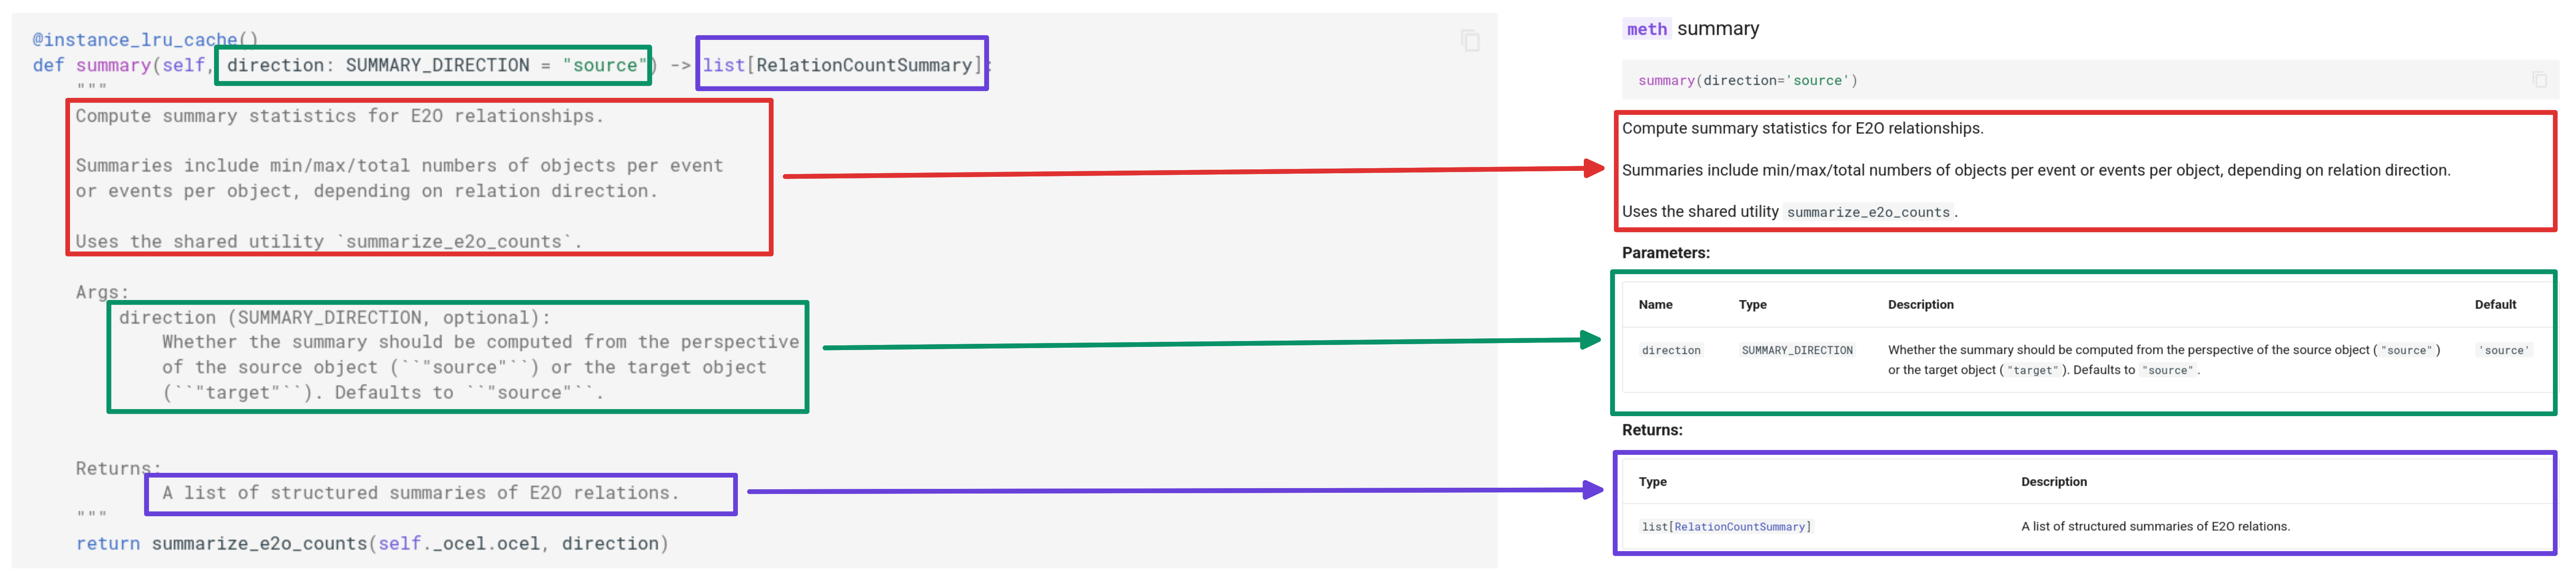
\includegraphics[width=\textwidth]{./figures/implementation/API Generation Example.png}
	\caption{Example of automatically generated API documentation.
		The API reference is derived from the source code, including docstrings, parameter descriptions, and return types.}
	\label{fig:doc-api-generation}
\end{figure}

\subsection{Automated Build and Release Process}

Ocelescope automates all build and release steps through workflows executed in GitHub Actions.
These workflows are defined through \texttt{.yml} files and are triggered by events such as code changes or new releases.
The documentation is deployed on every update, and the Python package is published whenever a release is created.

The main release task is the creation of the container images that make up Ocelescope.
Both the frontend and the backend are built as Docker images during each release.
A Dockerfile specifies how an image is created by installing dependencies, copying the code, and preparing the application.
The Dockerfiles also include steps that embed the modules of the system.

For the frontend image:

\begin{itemize}
	\item the API client is generated from the current OpenAPI schema,
	\item the frontend modules are embedded and the module router is created,
	\item all pages are statically generated to improve performance.
\end{itemize}

For the backend image:

\begin{itemize}
	\item backend modules are embedded into the image,
	\item the default OCELs are copied and enriched with metadata so that custom builds can replace or extend them.
\end{itemize}

The workflows use Docker Buildx to build native images for \texttt{amd64} and \texttt{arm64}.
This avoids performance issues that occur when running non-native images on arm64 systems.
The resulting images are pushed to Docker Hub.

This setup allows users who build on Ocelescope to release their own extensions for all common platforms without needing to understand the underlying build system.
